% This LaTeX document needs to be compiled with XeLaTeX.
\documentclass[10pt]{article}
\usepackage[utf8]{inputenc}
\usepackage{ucharclasses}
\usepackage{amsmath}
\usepackage{amsfonts}
\usepackage{amssymb}
\usepackage[version=4]{mhchem}
\usepackage{extpfeil}
\usepackage{stmaryrd}
\usepackage{bbold}
\usepackage{graphicx}
\usepackage[export]{adjustbox}
\graphicspath{ {./images/} }
\usepackage[fallback]{xeCJK}
\usepackage{polyglossia}
\usepackage{fontspec}
\IfFontExistsTF{Noto Serif CJK TC}
{\setCJKmainfont{Noto Serif CJK TC}}
{\IfFontExistsTF{STSong}
  {\setCJKmainfont{STSong}}
  {\IfFontExistsTF{Droid Sans Fallback}
    {\setCJKmainfont{Droid Sans Fallback}}
    {\setCJKmainfont{SimSun}}
}}

\setmainlanguage{vietnamese}
\setotherlanguages{english}
\newfontfamily\vietnamesefont{CMU Serif}
\IfFontExistsTF{CMU Serif}
{\newfontfamily\lgcfont{CMU Serif}}
{\IfFontExistsTF{DejaVu Sans}
  {\newfontfamily\lgcfont{DejaVu Sans}}
  {\newfontfamily\lgcfont{Georgia}}
}
\setDefaultTransitions{\lgcfont}{}
\setTransitionsFor{Vietnamese}{\vietnamesefont}{\lgcfont}

\begin{document}
\section*{ĐÁP ÁN VÀ HÚÓNG DẪN TRẢ LỜI}
\section*{BÀI 1}
1.1. a) (1) đồng thời; (2) chất sản phẩm; (3) chất phản ứng.\\
b) (1) bằng; (2) cân bằng động.\\
c) (1) lớn hơn; (2) các chất phản ứng.\\
1.2. $a-4, b-1, c-2, d-3$.\\
1.3. A.\\
1.4. D.\\
1.5. B.\\
1.6. a) (1) 617,166 ; (2) 0,3429 ; (3) 0,3376 .\\
$\mathrm{b}^{*}$ ) Khi nhiệt độ tăng, cân bằng chuyển dịch sang trái (theo chiều nghịch), do khi tăng nhiệt độ thì tạo ra nhiều $\mathrm{H}_{2}$ và $\mathrm{I}_{2}$ hơn.\\
1.7.C.\\
1.8. B.\\
$1.9^{*}$. B. Khi nén piston thì nồng độ, áp suất các chất đều tăng. Để hằng số cân bằng không đổi (do nhiệt độ không đổi) thì cân bằng phải chuyển dịch theo chiều thuận vì giá trị hằng số cân bằng phụ thuộc nhiều hơn vào nồng độ $\mathrm{N}_{2}$ và $\mathrm{H}_{2}$.\\
1.10. B.\\
1.11. A.\\
1.12. Học sinh tự viết.\\
1.13.

\begin{center}
\begin{tabular}{|l|l|l|l|l|}
\hline
 & $\mathrm{H}_{2}(\mathrm{~g})+$ & $\mathrm{I}_{2}(g)$ & $\rightleftharpoons$ & $2 \mathrm{HI}(g)$ \\
\hline
Nồng độ ban đầu (M) & 0,1040 & 0,1040 &  & 0 \\
\hline
Nồng độ phản ứng ( M ) & x & X &  & 2x \\
\hline
Nồng độ cân bằng (M) & 0,1040-x & 0,1040-x &  & 2x \\
\hline
\multicolumn{5}{|l|}{$[\mathrm{HI}]=2 \mathrm{x}=0,1924(\mathrm{M})$ suy ra $\mathrm{x}=0,0962(\mathrm{M})$.} \\
\hline
\multicolumn{5}{|l|}{$\left[\mathrm{H}_{2}\right]=\left[\mathrm{I}_{2}\right]=0,1040-0,0962=0,0078(\mathrm{M})$.} \\
\hline
\multicolumn{5}{|l|}{Vậy $\mathrm{K}_{\mathrm{C}}=608,4$.} \\
\hline
\end{tabular}
\end{center}

1.14*. a) Tuyến tuy có vai trò quan trọng trong việc ổn định lượng đường trong máu bởi tuyến này sản xuất hai loại hormone: insulin và glucagon. Hoạt động ăn uống sinḥ ra glucose, lúc này insulin sẽ có vai trò chuyển glucose thành glycogen tích trữ trong gan. Khi cơ thể hoạt động sẽ tiêu thụ glucose, lúc này glucagon sẽ có vai trò chuyển glycogen trong gan thành glucose.\\
b) Cả hai thời điểm đều xảy ra đồng thời hai quá trình sinh ra và mất đi glucose.

\begin{itemize}
  \item Khi hoạt động thể thao: tiêu hao glucose nhưng lại được sinh ra bổ sung từ glycogen.
  \item Khi ăn uống: sinh ra glucose do ăn uống và mất đi glucose do hoạt động của một số bộ phận (tay, miệng, não bộ,...).\\
Có thể coi đó là cân bằng hoá học đặc biệt do sự sinh ra và mất đi glucose liên quan đến các phản ứng hoá học. Ví dụ: Glucose $\rightleftharpoons$ Glycogen.\\
1.15. $\mathrm{K}_{\mathrm{C}}=\frac{[\mathrm{HbCO}]\left[\mathrm{O}_{2}\right]}{\left[\mathrm{HbO}_{2}\right][\mathrm{CO}]}$
\end{itemize}

$$
\frac{[\mathrm{HbCO}]}{\left[\mathrm{HbO}_{2}\right]}=\mathrm{K}_{\mathrm{C}} \frac{[\mathrm{CO}]}{\left[\mathrm{O}_{2}\right]}=170 \cdot \frac{0,10}{20,0}=0,85 .
$$

Nhận xét: Như vậy, mặc dù nồng độ CO rất nhỏ so với nồng độ $\mathrm{O}_{2}$ nhưng có thể làm một lượng đáng kể $\mathrm{HbO}_{2}$ chuyển thành HbCO , dẫn tới làm giảm khả năng vận chuyển $\mathrm{O}_{2}$ của máu một cách nghiêm trọng.

\section*{BÀI 2}
2.1. a) (1) sự điện li; (2) ion; (3) Chất không điện li.\\
b) (1) acid; (2) base; (3) hoàn toàn; (4) một phần.\\
2.2. A. $\mathrm{NaOH}, \mathrm{HCl}, \mathrm{HNO}_{3}, \mathrm{NaNO}_{3}, \mathrm{KAl}\left(\mathrm{SO}_{4}\right)_{2} \cdot 12 \mathrm{H}_{2} \mathrm{O}$.\\
2.3. C.\\
2.4.C.\\
2.5. A.\\
2.6. C.\\
2.7. D.\\
2.8. B.\\
2.9. A.\\
2.10. A.\\
2.11. D.\\
2.12. $\mathrm{NaHCO}_{3}(s) \xrightarrow{\mathrm{H}_{2} \mathrm{O}} \mathrm{Na}^{+}(a q)+\mathrm{HCO}_{3}^{-}(a q)$\\
$\mathrm{CuCl}_{2}(s) \quad \xrightarrow{\mathrm{H}_{2} \mathrm{O}} \mathrm{Cu}^{2+}(a q)+2 \mathrm{Cl}^{-}(a q)$\\
$\left(\mathrm{NH}_{4}\right)_{2} \mathrm{SO}_{4}(s) \xrightarrow{\mathrm{H}_{2} \mathrm{O}} 2 \mathrm{NH}_{4}^{+}(a q)+\mathrm{SO}_{4}^{2-}(a q)$\\
$\mathrm{Fe}\left(\mathrm{NO}_{3}\right)_{3}(s) \xrightarrow{\mathrm{H}_{2} \mathrm{O}} \mathrm{Fe}^{3+}(a q)+3 \mathrm{NO}_{3}^{-}(a q)$\\
2.13. $\mathrm{NaOH}(a q) \xrightarrow{\mathrm{H}_{2} \mathrm{O}} \mathrm{Na}^{+}(a q)+\mathrm{OH}^{-}(a q)$\\
$\mathrm{CH}_{3} \mathrm{OH}(l) \rightarrow \mathrm{CH}_{3} \mathrm{OH}(a q)$\\
Khi hoà tan vào nước, NaOH phân li hoàn toàn thành các ion, còn $\mathrm{CH}_{3} \mathrm{OH}$ không phân li mà tồn tại chủ yếu ở dạng phân tử.\\
2.14.

\begin{center}
\begin{tabular}{|l|l|l|}
\hline
Chát & Dạe điém & Dang tôn tai chú yéu trong dung dich nước \\
\hline
$\mathrm{CH}_{3} \mathrm{COOH}$ & Acid yếu & Phân tử $\mathrm{CH}_{3} \mathrm{COOH}$ \\
\hline
$\mathrm{HNO}_{3}$ & Acid mạnh & Ion $\mathrm{H}^{+}\left(\mathrm{H}_{3} \mathrm{O}^{+}\right)$và $\mathrm{NO}_{3}^{-}$ \\
\hline
$\mathrm{C}_{6} \mathrm{H}_{12} \mathrm{O}_{6}$ (glucose) & Chất không điện li & Phân tử $\mathrm{C}_{6} \mathrm{H}_{12} \mathrm{O}_{6}$ (glucose) \\
\hline
NaOH & Base mạnh & Ion $\mathrm{Na}^{+}$và $\mathrm{OH}^{-}$ \\
\hline
\end{tabular}
\end{center}

2.15. a) $\mathrm{H}^{+}(a q)+\mathrm{HCO}_{3}^{-}(a q) \rightarrow \mathrm{CO}_{2}(g)+\mathrm{H}_{2} \mathrm{O}$\\
b) $2 \mathrm{H}^{+}(a q)+\mathrm{Mg}(\mathrm{OH})_{2}(s) \rightarrow \mathrm{Mg}^{2+}(a q)+2 \mathrm{H}_{2} \mathrm{O}$\\
"Sữa magie" hiệu quả hơn nước bọt trong việc trung hoà acid thực quản do $\mathrm{Mg}(\mathrm{OH})_{2}$ là base mạnh hơn $\mathrm{HCO}_{3}^{-}$có trong nước bọt.\\
2.16. $\mathrm{H}_{2} \mathrm{SO}_{4}(a q) \rightarrow \mathrm{H}^{+}(a q)+\mathrm{HSO}_{4}^{-}(a q)$\\
$\mathrm{HSO}_{4}^{-}(a q) \rightleftharpoons \mathrm{H}^{+}(a q)+\mathrm{SO}_{4}^{2-}(a q)$\\
$\mathrm{HNO}_{3}(a q) \rightarrow \mathrm{H}^{+}(a q)+\mathrm{NO}_{3}^{-}(a q)$

\section*{BÀl 3}
3.1. (1) $1,0.10^{-14}$; (2) lớn hơn; (3) $1,0.10^{-7} \mathrm{M}$; (4) trung tính;\\
(5) $\left[\mathrm{OH}^{-}\right]$; (6) $1,0.10^{-7} \mathrm{M}$; (7) $1,0.10^{-7} \mathrm{M}$.\\
3.2. (d), (e), (g).\\
3.3. a, c, e-1; b, d, g-2.

Sử dụng acid mạnh thêm vào dung dịch trung tính để làm tăng tính acid. Dừng giấy chỉ thị acid - base để thử thấy màu giấy vàng đậm dần rồi sang đỏ nếu môi trường acid rất mạnh.\\
Sử dụng base mạnh thêm vào dung dịch trung tính để làm tăng tính base. Dừng giấy chỉ thị acid - base để thử thấy màu giấy chỉ thị acid - base xanh đậm dần rồi chuyển tím nếu môi trường base rất mạnh.\\
3.4. D.\\
3.5. (a), (e).\\
3.6. C.\\
3.7*。

\begin{center}
\begin{tabular}{|l|l|l|l|}
\hline
Durng dich & pH & Tinh acid, base hay trung tinh & Mau cua giây chí thi pH \\
\hline
A & 1 & Acid & Đỏ thẫm \\
\hline
B & 11 & Base & Xanh thẫm \\
\hline
C & 7 & Trung tinh & Xanh cốm \\
\hline
D & 3 & Acid & Vàng cam \\
\hline
E & 13 & Base & Xanh tím \\
\hline
F & 9 & Base & Xanh \\
\hline
\end{tabular}
\end{center}

3.8. Số $\mathrm{mol} \mathrm{H}^{+}$trong 50 mL HBr là: $0,05 \cdot 0,050=2,5 \cdot 10^{-3}(\mathrm{~mol})$.

Số $\mathrm{mol} \mathrm{H}^{+}$trong 150 mL HI là: $0,15 \cdot 0,100=1,5 \cdot 10^{-2}(\mathrm{~mol})$.\\
Nồng độ $\mathrm{H}^{+}$của đúng dịch X là:

$$
\left[\mathrm{H}^{+}\right]=\frac{2,5 \cdot 10^{-3}+1,5 \cdot 10^{-2}}{0,05+0,15}=0,0875(\mathrm{M}) ; \mathrm{pH}=-\lg (0,0875)=1,06
$$

3.9. Số mol NaOH thêm vào là $2,5 \cdot 10^{-3} \mathrm{~mol}$; số mol HCl ban đầu là $5 \cdot 10^{-3} \mathrm{~mol}$.

Dựa vào phương trình $\mathrm{H}^{+}+\mathrm{OH}^{-} \rightarrow \mathrm{H}_{2} \mathrm{O}$, tính được số mol $\mathrm{H}^{+}$trong dung dịch thu được sau khi thêm NaOH là $2,5 \cdot 10^{-3} \mathrm{~mol}$.\\
Vậy $\mathrm{pH}=-\lg \left(\frac{2,5 \cdot 10^{-3}}{0,025+0,05}\right)=1,48$.\\
3.10. Nồng độ $\mathrm{OH}^{-1}$ là: $\frac{10^{-14}}{10^{-10,66}}=10^{-3,34}=4,57.10^{-4}(\mathrm{M})$.

Nồng độ của $\mathrm{Ba}(\mathrm{OH})_{2}$ tương ứng là: $2,285 \cdot 10^{-4} \mathrm{M}$.\\
Để thu được 125 mL dung dịch $\mathrm{Ba}(\mathrm{OH})_{2}$ thì khối lượng $\mathrm{Ba}(\mathrm{OH})_{2}$ cần hoà tan là:\\
$2,285 \cdot 10^{-4} \cdot 125 \cdot 10^{-3} \cdot 171=4,884 \cdot 10^{-3}(\mathrm{~g})$.\\
3.11. C. Cả hydrochloric acid và ethanoic acid (acetic acid) đều là acid đơn chức nên khi các thể tích và nồng độ bằng nhau của các acid này được chuẩn độ bằng sodium hydroxide thì cần cùng một thể tích base để đạt đến điểm tương dưong.\\
3.12. a) B; b) A.\\
3.13. Phương trình hoá học của các phản ứng xảy ra như sau:

$$
\begin{aligned}
& 2 \mathrm{NaOH}+\mathrm{H}_{2} \mathrm{SO}_{4} \rightarrow \mathrm{Na}_{2} \mathrm{SO}_{4}+2 \mathrm{H}_{2} \mathrm{O} \\
& \mathrm{HCl}+\mathrm{NaOH} \rightarrow \mathrm{NaCl}+\mathrm{H}_{2} \mathrm{O}
\end{aligned}
$$

Số mol NaOH thêm vào 100 mL dung dịch $\mathrm{H}_{2} \mathrm{SO}_{4}$ là: $0,05 \cdot 0,213=1,065 \cdot 10^{-2}(\mathrm{~mol})$.\\
Số mol NaOH được trung hoà bởi HCl là: $0,01321 \cdot 0,103=1,361 \cdot 10^{-3}(\mathrm{~mol})$.\\
Số mol NaOH được trung hoà bởi 100 mL dung dịch $\mathrm{H}_{2} \mathrm{SO}_{4}$ là:\\
$1,065 \cdot 10^{-2}-1,361 \cdot 10^{-3}=9,289 \cdot 10^{-3}(\mathrm{~mol})$.\\
Vậy nồng độ $\mathrm{H}_{2} \mathrm{SO}_{4}$ trong mẫu phân tích là: $\frac{9,289 \cdot 10^{-3}}{2 \cdot 0,1}=0,0464(\mathrm{M})$.\\
3.14. a) Acid đó là acid hai lần acid.\\
b) Base có khả năng nhận 2 proton (chứa hai nhóm -OH ). Ví dụ $\mathrm{Ca}(\mathrm{OH})_{2}$, $\mathrm{Ba}(\mathrm{OH})_{2}$.\\
3.15*. a) a1) $\left[\mathrm{H}^{+}\right]=2 \cdot 5 \cdot 10^{-3}=10^{-2}(\mathrm{M}) ; \mathrm{pH}=-\lg \left(10^{-2}\right)=2$.\\
a2) $\mathrm{pH}=3$ vì dung dịch được pha loãng 10 lần.\\
b) Phương trình hoá học của phản ứng xảy ra:

$$
\mathrm{H}_{2} \mathrm{SO}_{4}+2 \mathrm{NaOH} \rightarrow \mathrm{Na}_{2} \mathrm{SO}_{4}+2 \mathrm{H}_{2} \mathrm{O}
$$

c) c1) Nhỏ 1 giọt phenolphthalein vào dung dịch NaOH , dung dịch có màu hồng. Chuẩn độ bằng dung dịch $\mathrm{H}_{2} \mathrm{SO}_{4}$, màu hồng sẽ nhạt dần, khi đạt tới điểm tương đương sẽ mất màu.\\
c2) Thể tích dung dịch acid cần dùng là:

$$
25 \cdot 1,00 \cdot 10^{-4}: \frac{2 \cdot 5 \cdot 10^{-3}}{10}=2,5(\mathrm{~mL})
$$

3.16*. Khí carbon dioxide tan trong nước theo phương trình hoá học sau:

$$
\begin{aligned}
& \mathrm{CO}_{2}(g)+\mathrm{H}_{2} \mathrm{O}(l) \rightleftharpoons \mathrm{H}_{2} \mathrm{CO}_{3}(a q) \\
& \mathrm{H}_{2} \mathrm{CO}_{3}(a q)+\mathrm{H}_{2} \mathrm{O}(l) \rightleftharpoons \mathrm{HCO}_{3}^{-}(a q)+\mathrm{H}_{3} \mathrm{O}^{+}(a q)
\end{aligned}
$$

Nếu con người tiếp tục phát thải $\mathrm{CO}_{2}$, các cân bằng trên chuyển dịch tạo ra nhiều $\left[\mathrm{H}^{+}\right]$hon, làm pH của nước biển giảm, tức là nước biển càng bị acid hoá. Điều này ảnh hưởng đến môi trường sinh sống của các sinh vật biển. Nếu pH của nước biển càng thấp có thể dẫn đến sự hoà tan của các rạn san hô, vỏ sò, vỏ hàu,...\\
3.17*: Oxygen được dẫn truyền trong cơ thể là do khả năng liên kết của oxygen với hồng cầu trong máu theo cân bằng sau:


\begin{equation*}
\mathrm{HbH}^{+}(a q)+\mathrm{O}_{2}(a q) \rightleftharpoons \mathrm{HbO}_{2}(a q)+\mathrm{H}^{+}(a q) \tag{1}
\end{equation*}


Theo nguyên lí chuyển dịch cân bằng Le Chatelier, nếu nồng độ $\mathrm{H}^{+}$tăng, cân bằng (1) sẽ chuyển dịch sang trái; nếu nồng độ $\mathrm{H}^{+}$giảm, cân bằng (1) sẽ chuyển dịch sang phải. Vì vậy, nếu pH của máu quá thấp (nồng độ $\mathrm{H}^{+}$cao), cân bằng sẽ chuyển dịch sang trái. Điều này khiến trong máu có it $\mathrm{HbO}_{2}$, nên khả năng vận chuyển oxygen của hồng cầu sẽ giảm.\\
3.18. a) Acid yếu khồng phân li hoàn toàn;

$$
\mathrm{CH}_{3} \mathrm{COOH}+\mathrm{H}_{2} \mathrm{O}=\mathrm{CH}_{3} \mathrm{COO}^{-}+\mathrm{H}_{3} \mathrm{O}^{+}
$$

b) $2 \mathrm{CH}_{3} \mathrm{COOH}+\mathrm{CaCO}_{3} \rightarrow \mathrm{Ca}\left(\mathrm{CH}_{3} \mathrm{COO}\right)_{2}+\mathrm{CO}_{2}+\mathrm{H}_{2} \mathrm{O}$

\section*{BÀI 4}
4.1. B.\\
4.2. B.\\
4.3. A.\\
4.4. a) A; b) C; c) A; d) C; e) A; g) D.\\
4.5. (a), (b), (d).\\
4.6*. Dựa trên tính chất là khí nitrogen không duy trì sự cháy, gần như trơ ở nhiệt độ thường và nhiệt độ không quá cao (chỉ hoạt động ở nhiệt độ rất cao) nên nitrogen được dùng trong phòng cháy, chữa cháy; bảo quản thực phẩm, ngăn thực phẩm bị oxi hoá nhanh hỏng; ngăn ethanol trong bia bị oxi hoá thành acid gây ra vị chua. Nitrogen lỏng có nhiệt độ rất thấp $-196^{\circ} \mathrm{C}$. Ngoài giúp trữ đông mô, việc đưa một lượng khí nitrogen ở nhiệt độ rất thấp vào mô ung thư có thể làm đông đặc mô bệnh, sau đó rã đông, quá trình lặp lại nhiều lần mô bệnh sẽ chết và được loại bỏ; phương pháp này ít gây đau đớn và ít mất máu cho bệnh nhân hơn so với phẫu thuật truyền thống.\\
4.7. a) $\triangle_{\mathrm{r}} \mathrm{H}_{298}^{\mathrm{o}}=1.946+3.436-6.389=-80(\mathrm{~kJ})$.\\
b) Với kết quả tính được từ a) thì enthalpy tạo thành chuẩn của ammonia là $-40 \mathrm{~kJ} \mathrm{~mol}^{-1}$.\\
c) Giá trị enthalpy tạo thành chuần tính theo năng lượng liên kết thường khác biệt nhiều với giá trị thực nghiệm. Đó là do giá trị năng lượng của một liên kết cộng hoá trị giữa A và B thường chỉ là giá trị năng lượng liên kết trung bình của các liên kết giữa A và B trong nhiều hợp chất khác nhau. Trong bài tập này, giá trị $389 \mathrm{~kJ} \mathrm{~mol}^{-1}$ được hiểu là giá trị trung bình năng lượng liên kết N và H trong nhiều hợp chất khác nhau, như $\mathrm{NH}_{3}, \mathrm{CH}_{3}-\mathrm{NH}_{2}, \ldots$

\section*{BÀ1 5}
5.1. $a-3 ; b-1,2,4 ; c-5,6$.\\
5.2. B.\\
5.3. (a), (b), (e), (g).\\
5.4. a) Giảm.\\
b) Theo nguyên lí chuyển dịch cân bằng Le Chatelier, khi nhiệt độ tăng thì cân bằng chuyển dịch theo chiều phản ứng thu nhiệt, tức phản ứng nghịch. Điều đó làm giảm hiệu suất thu ammonia.\\
c) Theo nguyên lí chuyển dịch cân bằng Le Chatelier, khi áp suất tăng thì cân bằng chuyển dịch theo chiều làm giảm áp suất, trúc chiều giảm số mol khí, chiều thuận. Điều đó làm tăng hiệu suất thu ammonia.\\
d) Khoảng $400^{\circ} \mathrm{C}$.\\
5.5. - Quá trình sản xuất $\mathrm{NH}_{4} \mathrm{Cl}, \mathrm{NH}_{4} \mathrm{NO}_{3},\left(\mathrm{NH}_{4}\right)_{2} \mathrm{SO}_{4}$ theo phản úng trực tiếp giữa ammonia và acid tương úng; đó không phải là các phản úng oxi hoá - khử.

\begin{itemize}
  \item Quá trình sản xuất urea theo phản ứng:
\end{itemize}

$$
2 \mathrm{NH}_{3}+\mathrm{CO}_{2} \xlongequal{\mathrm{t}^{\circ}, \mathrm{p}}\left(\mathrm{NH}_{2}\right)_{2} \mathrm{CO}+\mathrm{H}_{2} \mathrm{O}
$$

Đây không phải là phản ứng oxi hoá - khử.

\begin{itemize}
  \item Các phản ứng trên không tạo khí độc. Tuy nhiên khi sử dụng dư thừa, phân bón chứa các chất này sẽ gây hiện tượng phú dưỡng cho nước và đất.\\
5.6. a) Mức thuỷ ngân trong ống nghiệm chựa urea sẽ thấp hơn do quá trình hoà tan urea thu nhiều nhiệt hơn.\\
b) Có thể phân biệt được dựa vào nhiệt hoà tan.\\
5.7. B. Công thức (2) và (5) không thoả mãn quy tắc octet.\\
5.8. a) Có 1 cặp electron hoá trị ghép đôi, 3 electron hoá trị độc thân.\\
b) b1) Công thức (A) phù hợp hơn vì nguyên tử N chỉ có 4 orbital hoá trị, do đó chỉ có thể tạo tối đa 4 liên kết cộng hoá trị. Theo công thức (A), N có hoá trị là IV và số oxi hoá là +5 .\\
$\left.\mathrm{b} 2^{*}\right)$ Công thức $(\mathrm{A})$ phù hợp với dữ liệu do có ba loại liên kết giữa N và O không tương đương nhau trong phân tứ $\mathrm{HNO}_{3}$ ( 1 liên kết đôi, 1 liên kết đơn theo kiểu ghép đôi electron hoá trị và 1 liên kết đơn theo kiểu cho - nhận).\\
5.9. Phân ammonium nitrate có nguy cơ cháy, nổ cao hơn, do phản ứng phân huỷ phát nhiều nhiệt. Ví dụ, vụ nổ ở Beirut, Lebanon (Li-băng) năm 2020 làm hàng trăm người chết; hàng trăm nghìn người mât nhà cưa; nguyên nhân được cho là liên quan đến 2750 tấn ammonium nitrate được cất giự ở cảng suốt 6 năm một cách không an toàn. Vụ nổ có sức công phá tương đương 1200 tấn thuốc nổ TNT.\\
5.10. a) $4 \mathrm{C}_{6} \mathrm{H}_{10} \mathrm{O}+6 \mathrm{HNO}_{3} \rightarrow 4 \mathrm{C}_{6} \mathrm{H}_{10} \mathrm{O}_{4}+3 \mathrm{~N}_{2} \mathrm{O}+3 \mathrm{H}_{2} \mathrm{O}$\\
b) Do số oxi hoá của N đă giảm từ +5 (trong $\mathrm{HNO}_{3}$ ) xuống +1 (trong $\mathrm{N}_{2} \mathrm{O}$ ) nên $\mathrm{HNO}_{3}$ đóng vai trò chất oxi hoá.\\
5.11. a) $\mathrm{Au}+\mathrm{HNO}_{3}+4 \mathrm{HCl} \rightarrow \mathrm{HAuCl}_{4}+2 \mathrm{H}_{2} \mathrm{O}+\mathrm{NO}$\\
b) Do số oxi hoá của N đã giảm từ +5 (trong $\mathrm{HNO}_{3}$ ) xuống +2 (trong NO ) nên $\mathrm{HNO}_{3}$ đóng vai trò chất oxi hoá.
\end{itemize}

\section*{BÀl 6}
6.1. (a), (c) và (d).\\
6.2. a) Các liên kết $\mathrm{S}-\mathrm{S}$ trong $\mathrm{S}_{8}$ đều là liên kết cộng hoá trị không cực nên hợp chất $\mathrm{S}_{8}$ cũng là hợp chất không phân cực.\\
b) (b1), (b3).\\
6.3. Khí thiên nhiên và than khi cháy sẽ toả rất nhiều nhiệt, tạo điều kiện cho các hợp chất như hydrogen sulfide và các hợp chất chứa $\mathrm{S}, \mathrm{N}$ bị oxi hoá sinh ra các khí độc gây ô nhiễm như $\mathrm{SO}_{2}, \mathrm{NO}, \mathrm{NO}_{2}, \ldots$, các khí này là nguyên nhân gây mưa acid. Ví dụ: $2 \mathrm{H}_{2} \mathrm{~S}(g)+3 \mathrm{O}_{2}(g) \xrightarrow{\mathrm{t}^{\mathrm{e}}} 2 \mathrm{SO}_{2}(g)+2 \mathrm{H}_{2} \mathrm{O}(l)$\\
6.4. (a), (c).\\
6.5. $a-2,4,6 ; b-1,3,5,6$.\\
6.6. a) $\mathrm{SO}_{2}+\mathrm{H}_{2} \mathrm{O} \rightleftharpoons \mathrm{H}_{2} \mathrm{SO}_{3}$\\
b) $\mathrm{SO}_{2}+2 \mathrm{NaOH} \rightarrow \mathrm{Na}_{2} \mathrm{SO}_{3}+\mathrm{H}_{2} \mathrm{O}$\\
c) $\mathrm{SO}_{2}+\mathrm{CaO} \rightarrow \mathrm{CaSO}_{3}$\\
6.7. Giá trị biến thiên enthalpy chuẩn của phản ứng là:

$$
\Delta_{\mathrm{r}} \mathrm{H}_{298}^{\circ}=(-395,7)-(-296,8)=-98,9(\mathrm{~kJ})
$$

Giá trị biến thiên enthalpy chuẩn của phản ứng có giá trị âm, tức phản ứng toả nhiệt nên thuận lợi về mặt năng lượng.\\
6.8. a) Cả hai phản ứng đều thuận lợi về mặt năng lượng vì giá trị biến thiên enthalpy chuẩn của hai phản ứng đều âm (-517,9 kJ và -221,1 kJ).\\
b) Hydrogen sulfide sẽ dễ chuyển thành sulfur dioxide theo phản ứng (2), vì phản ứng (2) cần ít oxygen hơn so với phản ứng (1).\\
6.9. a) Vi S trong khí thải ( $\mathrm{SO}_{2}$ ) được thay thế bằng C (trong $\mathrm{CO}_{2}$ ).\\
b) $\Delta_{\mathrm{r}} \mathrm{H}_{298}^{0}=-524,0 \mathrm{~kJ}$. Phản ứng toả nhiệt nên thuận lợi về năng lượng.\\
c) Để tăng diện tích tiếp xúc giữa calcium carbonate với khí nhằm tăng tốc độ phản úng.\\
d) Là phản ứng oxi hoá - khử vì làm tăng số oxi hoá của suîfur từ +4 (trong $\mathrm{CaSO}_{3}$ ) lên +6 (trong $\mathrm{CaSO}_{4}$ ).

\section*{BAI 7}
7.1. (a), (c).\\
7.2. (a), (c), (d).\\
7.3. $\mathrm{a}-1,4,5,6 ; \mathrm{b}-2,3 ; \mathrm{c}-1,2,4,5$.\\
7.4. a) Do 6 electron hoá trị của S bị lệch về phía các nguyên tử O nên S có số oxi hoá là +6.\\
b) S chỉ có 6 electron hoá trị nên không thể có số oxi hoá lớn hơn 6.\\
c) $8 \mathrm{HI}+\mathrm{H}_{2} \mathrm{SO}_{4} \rightarrow \mathrm{H}_{2} \mathrm{~S}+4 \mathrm{I}_{2}+4 \mathrm{H}_{2} \mathrm{O}$.\\
7.5. a) Lớp oxide tan dần, sau đó lá kim loại cũng tan và có bọt khí xuất hiện.

$$
\begin{aligned}
& \mathrm{H}_{2} \mathrm{SO}_{4}(a q)+\mathrm{ZnO}(s) \rightarrow \mathrm{ZnSO}_{4}(a q)+\mathrm{H}_{2} \mathrm{O}(l) \\
& \mathrm{H}_{2} \mathrm{SO}_{4}(a q)+\mathrm{Zn}(s) \rightarrow \mathrm{ZnSO}_{4}(a q)+\mathrm{H}_{2}(g)
\end{aligned}
$$

b) Mẩu đá vôi tan ra, dung dịch sủi bọt khí, dung dịch sau phản ứng có màu trắng đục, để lâu sẽ lắng thành lớp bột màu trắng.

$$
\mathrm{H}_{2} \mathrm{SO}_{4}(a q)+\mathrm{CaCO}_{3}(s) \rightarrow \mathrm{CaSO}_{4}(s)+\mathrm{CO}_{2}(g)+\mathrm{H}_{2} \mathrm{O}(l)
$$

c) Bột baking soda tan ra, dung dịch sủi bọt khí, sau phản ứng thu được dung dịch trong suốt.

$$
\mathrm{H}_{2} \mathrm{SO}_{4}(a q)+2 \mathrm{NaHCO}_{3}(s) \rightarrow \mathrm{Na}_{2} \mathrm{SO}_{4}(a q)+2 \mathrm{CO}_{2}(g)+2 \mathrm{H}_{2} \mathrm{O}(l)
$$

d) Nước vôi trong bị đục.

$$
\mathrm{H}_{2} \mathrm{SO}_{4}(a q)+\mathrm{Ca}(\mathrm{OH})_{2}(a q) \rightarrow \mathrm{CaSO}_{4}(s)+2 \mathrm{H}_{2} \mathrm{O}(l)
$$

7.6. a) $2 \mathrm{H}_{2} \mathrm{SO}_{4}+\mathrm{C} \rightarrow \mathrm{CO}_{2}+2 \mathrm{SO}_{2}+2 \mathrm{H}_{2} \mathrm{O}$\\
b) $\mathrm{SO}_{2}+\mathrm{Br}_{2}+2 \mathrm{H}_{2} \mathrm{O} \rightarrow 2 \mathrm{HBr}+\mathrm{H}_{2} \mathrm{SO}_{4}$\\
c) $5 \mathrm{SO}_{2}+2 \mathrm{KMnO}_{4}+2 \mathrm{H}_{2} \mathrm{O} \rightarrow 2 \mathrm{MnSO}_{4}+\mathrm{K}_{2} \mathrm{SO}_{4}+2 \mathrm{H}_{2} \mathrm{SO}_{4}$\\
d) $2 \mathrm{H}_{2} \mathrm{SO}_{4}+2 \mathrm{FeSO}_{4} \rightarrow \mathrm{Fe}_{2}\left(\mathrm{SO}_{4}\right)_{3}+\mathrm{SO}_{2}+2 \mathrm{H}_{2} \mathrm{O}$\\
e) $8 \mathrm{H}_{2} \mathrm{SO}_{4}+10 \mathrm{FeSO}_{4}+2 \mathrm{KMnO}_{4} \rightarrow 5 \mathrm{Fe}_{2}\left(\mathrm{SO}_{4}\right)_{3}+\mathrm{K}_{2} \mathrm{SO}_{4}+2 \mathrm{MnSO}_{4}+8 \mathrm{H}_{2} \mathrm{O}$\\
g) $8 \mathrm{H}^{+}+5 \mathrm{Fe}^{2+}+\mathrm{MnO}_{4}^{-} \rightarrow 5 \mathrm{Fe}^{3+}+\mathrm{Mn}^{2+}+4 \mathrm{H}_{2} \mathrm{O}$\\
7.7. a) Goi ý:

\begin{itemize}
  \item Baking soda: làm bánh,...
  \item Thạch cao nung: đúc tượng,...
  \item Phèn chua: làm trong nước, tạo môi trường acid nhẹ.\\
b) Hoà tan một lượng nhỏ mỗi chất trên vào nước, chất không tan là thạch cao. Để yên dung dịch hai chất hoà tan một thời gian, dung dịch nào xuất hiện chất keo là phèn nhôm kali.
\end{itemize}

$$
\begin{aligned}
& \mathrm{Al}^{3+}(a q)+\mathrm{H}_{2} \mathrm{O}(l) \rightleftharpoons \mathrm{Al}(\mathrm{OH})^{2+}(a q)+\mathrm{H}^{+}(a q) \\
& \mathrm{Al}(\mathrm{OH})^{2+}(a q)+\mathrm{H}_{2} \mathrm{O}(l) \rightleftharpoons \mathrm{Al}(\mathrm{OH})_{2}^{+}(a q)+\mathrm{H}^{+}(a q) \\
& \mathrm{Al}(\mathrm{OH})_{2}^{+}(a q)+\mathrm{H}_{2} \mathrm{O}(l) \rightleftharpoons \mathrm{Al}(\mathrm{OH})_{3}(s)+\mathrm{H}^{+}(a q)
\end{aligned}
$$

c) Dưng nước hoà tan các mẫu bột mịn tạo thành dung dịch, thạch cao nung tan khá ít. Có thể dùng quỳ tím để nhận biết nhanh hơn hai dung dịch còn lại, dung dịch làm quỳ hoá xanh là baking soda, hoá đỏ là phèn nhôm kali. Do dung dịch baking soda có quá trình:

$$
\mathrm{HCO}_{3}^{-}(a q)+\mathrm{H}_{2} \mathrm{O}(l) \rightleftharpoons \mathrm{H}_{2} \mathrm{CO}_{3}(a q)+\mathrm{OH}^{-}(a q)
$$

Và dung dịch phèn nhôm kali tạo môi trường acid như đã nêu ở ý b).\\
7.8. a) (1) $4 \mathrm{FeS}_{2}(s)+11 \mathrm{O}_{2}(g) \xrightarrow{t^{\circ}} 2 \mathrm{Fe}_{2} \mathrm{O}_{3}(s)+8 \mathrm{SO}_{2}(g)$\\
(2) $2 \mathrm{SO}_{2}(g)+\mathrm{O}_{2}(g) \xlongequal{450^{\circ} \mathrm{C}, \mathrm{V}_{2} \mathrm{O}_{5}} 2 \mathrm{SO}_{3}(g)$\\
(3) $\mathrm{H}_{2} \mathrm{SO}_{4}(a q)+\mathrm{nSO}_{3}(g) \rightarrow \mathrm{H}_{2} \mathrm{SO}_{4} \cdot \mathrm{nSO}_{3}(l)$\\
(4) $\mathrm{H}_{2} \mathrm{SO}_{4} \cdot \mathrm{nSO}_{3}(l)+\mathrm{nH}_{2} \mathrm{O}(l) \rightarrow(\mathrm{n}+1) \mathrm{H}_{2} \mathrm{SO}_{4}(a q)$\\
b) Phản ứng (2) toả nhiệt. Để cân bằng chuyển dịch theo chiều tạo ra nhiều sản phẩm hơn (chiều thuận), phản ứng nên được thực hiện ở nhiệt độ thấp. Tuy nhiên, thực tế phản ứng được thực hiện ở nhiệt độ cao nhằm tăng tốc độ phản ứng, tăng hiệu quả tạo thành sản phẩm trong một khoảng thời gian nhất định.\\
c) C. Lợi dựng tác dụng của trọng lực, $\mathrm{SO}_{3}(g)$ là chất khí, xả vào từ bên dưới sẽ tự khuếch tán lên trên; $\mathrm{H}_{2} \mathrm{SO}_{4}(a q)$ là chất lòng được phun dưới dạng sương rơi từ trên xuống ngược chiều với $\mathrm{SO}_{3}(g)$ làm tăng hiệu quả tiếp xúc.\\
d) $\quad \mathrm{H}_{2} \mathrm{SO}_{4} \mathrm{nSO}_{3}(l)+\mathrm{nH}_{2} \mathrm{O}(l) \rightarrow(\mathrm{n}+1) \mathrm{H}_{2} \mathrm{SO}_{4}(a q)$

$$
\mathrm{x} \quad(\mathrm{n}+1) \mathrm{x} \quad(\mathrm{~mol})
$$

Số $\mathrm{mol} \mathrm{H}_{2} \mathrm{SO}_{4}$ trong dung dịch sau pha loãng là:

$$
\frac{20,01 \cdot 0,10}{2 \cdot 10,0} \cdot 1,0=(\mathrm{n}+1) \mathrm{x}
$$

$\Rightarrow 0,10=(\mathrm{n}+1) \cdot \frac{8,36}{98+80 \mathrm{n}} \Rightarrow \mathrm{n}=4$. Vậy công thức của oleum là $\mathrm{H}_{2} \mathrm{SO}_{4} \cdot 4 \mathrm{SO}_{3}$.\\
7.9. a) Khối lượng CuO trong 1 tấn nguyên liệu là: $1000.96 \%=960(\mathrm{~kg})$.

Theo so đồ $\mathrm{CuO} \rightarrow \mathrm{CuSO}_{4} \cdot 5 \mathrm{H}_{2} \mathrm{O}$\\
Khối lượng copper(II) sulfate pentahydrate rắn thu được với hiệu suất $100 \%$ là:

$$
\frac{960}{80} .250=3000(\mathrm{~kg})
$$

Khối lượng copper(II) sulfate pentahydrate rắn thu được với hiệu suất $85 \%$ là:

$$
3000.85 \%=2550(\mathrm{~kg})
$$

b) Thể tích nước trong ao là:

$$
2000 \cdot 0,7=1400\left(\mathrm{~m}^{3}\right)
$$

Khối lượng copper(II) sulfate pentahydrate người dân cần sử dụng là:

$$
1400.0,25.3=1050(\mathrm{~g})=1,050 \mathrm{~kg} .
$$

c) $\mathrm{n}_{\mathrm{CuSO}_{4} \cdot 5 \mathrm{H}_{2} \mathrm{O}}=\mathrm{n}_{\mathrm{CuSO}_{4}}=10^{-4} \cdot 1=10^{-4}(\mathrm{~mol})$.

Vậy khối lượng của $\mathrm{CuSO}_{4} \cdot 5 \mathrm{H}_{2} \mathrm{O}$ là: $10^{-4} \cdot 250=0,0250(\mathrm{~g})=25,0 \mathrm{mg}$.

\section*{BÀI 8}
8.1. (b), (c), (e), (g). 8.2. C. 8.3. C.\\
8.4.C. 8.5.A. 8.6.D.\\
8.7. A có nhóm chức carboxylic acid, B có nhóm chức alcohol và D có nhóm chức ketone.\\
8.8. a) (1) là chuyển hoá giữa hai chất vô cơ.\\
b) (3) là chuyển hoá giữa hai chất hữu cơ.\\
c) (2) là chuyển hoá từ chất vô cơ thành chất hữu cơ.\\
8.9. a) Chất lỏng trong ống chữ U là nước. Do trong thành phần của alkane có hydrogen, khi đốt cháy tạo thành nước (hơi). Hơi nước gặp lạnh bị ngưng tụ tạo thành chất lỏng không màu. Nước đá có tác dụng làm lạnh để ngưng tụ hơi nước.\\
b) Trong thành phần của alkane có carbon, khi bị đốt cháy tạo thành khí carbon dioxide. Khí carbon dioxide phản ứng với nước vôi trong tạo thành $\mathrm{CaCO}_{3}$ không tan, làm vẩn đục nước vôi trong:

$$
\mathrm{CO}_{2}+\mathrm{Ca}(\mathrm{OH})_{2} \rightarrow \mathrm{CaCO}_{3}+\mathrm{H}_{2} \mathrm{O}
$$

c) Thí nghiệm trên tạo thành $\mathrm{H}_{2} \mathrm{O}$ và $\mathrm{CO}_{2}$, chứng tỏ trong thành phần của alkane bị đốt cháy có chứa các nguyên tố C và H .\\
8.10. a) Dẫn sản phẩm cháy qua ống chứa $\mathrm{Cu}(\mathrm{OH})_{2}$ khan (màu trắng), sự xuất hiện của $\mathrm{Cu}(\mathrm{OH})_{2} \cdot 5 \mathrm{H}_{2} \mathrm{O}$ (màu xanh) chứng tỏ trong sản phẩm cháy có $\mathrm{H}_{2} \mathrm{O}$. Tiếp tục dẫn sản phẩm cháy qua ống nước vôi trong (chứa $\mathrm{Ca}(\mathrm{OH})_{2}$ ), sự xuất hiện của $\mathrm{CaCO}_{3}$ (khiến nước vôi trong vẩn đục) chứng tỏ trong sản phẩm cháy có $\mathrm{CO}_{2}$.\\
b) Nguyên tố chắc chắn có mặt trong chất A là C và H . Nguyên tố có thể có trong chất A là O .

Để biết chắc chắn có hay không có $O$ trong chất $A$, cần so sánh lượng oxygen dùng để đốt cháy chất A và lượng oxygen có trong sản phẩm cháy $\left(\mathrm{CO}_{2}\right.$ và $\left.\mathrm{H}_{2} \mathrm{O}\right)$ : Nếu tổng khối lượng oxygen có trong sản phẩm cháy lớn hơn khối lượng oxygen dùng đốt cháy chất A cho phép kết luận trong chất A có oxygen; nếu lượng oxygen bằng nhau thì trong chất A không có oxygen.\\
c) Trên phổ IR của A thấy có hấp thụ ở $1720 \mathrm{~cm}^{-1}$ chứng tỏ trong phân tử chất A có thể có nhóm chức carboxylic acid hoặc ester hoặc ketone hoặc aldehyde.\\
8.11. Alà chất (3) do trên phổIR của A có hấp thựở $3281 \mathrm{~cm}^{-1}$, là tín hiệu đặc trưng cho liên kết $\mathrm{N}-\mathrm{H}$ trong phân tử amine; đồng thời không có hấp thự trong vùng $1750-1670 \mathrm{~cm}^{-1}$, là tín hiệu đặc trưng cho hấp thụ của liên kết $\mathrm{C}=\mathrm{O}$ trong các phân tử carboxylic acid (chất (1)), aldehyde (chất (2)) hay ketone (chất (4)).\\
8.12. a) Các nhóm chức acid hoặc ester được khoanh:\\
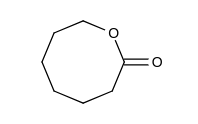
\includegraphics{smile-5b3cdc53965d017086e900b2b1f31e650836f869}

formic acid\\
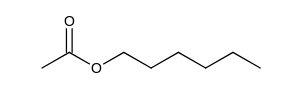
\includegraphics{smile-b389954ca42e6eadd69f6f9e9ae6773999a21ae6}

acetic acid\\
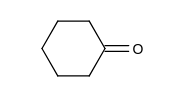
\includegraphics{smile-9410f9e408d3f9a7da6c439d17e79f6a7b7f10e7}

methyl formate\\
b) Do trong phân tử formic acid và methyl formate có nhóm chức aldehyde nên chúng thể hiện được tính chất của một aldehyde.\\
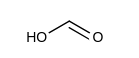
\includegraphics{smile-fe0a767c7ec10697c898ad9be9abfe6a2ffccd59}

formic acid\\
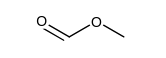
\includegraphics{smile-11bdff789f95735f92506e97e848eb5871f1919b}

methyl formate

\section*{BÀl 9}
9.1. B.\\
9.2. B.\\
9.3. A.\\
9.4. C.\\
9.5. D.\\
9.6. B.\\
9.7.B.\\
9.8. Các hợp chất hoá học có sẵn trong tự nhiên hoặc tạo thành trong các phản ứng hoá học thường không ở dạng tinh khiết mà lẫn với chất khác. Cô lập và tinh chế nhằm có được chất mong muốn ở dạng tinh khiết.\\
Một số phương pháp dùng tinh chế chất hữu cơ: phương pháp kết tinh, phương pháp chiết, phương pháp chưng cất, phương pháp sắc kí,...\\
Ví dụ: - Dể có được đường saccharose, người ta lấy nước ép mía đem cô đặc rồi kết tinh để được tinh thể đường.

\begin{itemize}
  \item Để có được rượu (dung dịch ethanol) từ hỗn hợp lên men của "cơm rượu", người ta tiến hành chưng cất lấy rượu khỏi phần "bã rượu".\\
-Để có được các hoạt chất từ thảo mộc để chữa bệnh, người ta lấy thảo mộc ngâm rượu uống (chiết các hoạt chất tan vào rượu) hoặc đun sôi với nước.\\
9.9. a) Phương pháp sử dụng để thu lấy iodine từ dung dịch iodine trong nước là phương pháp chiết lỏng - lỏng.\\
b) Dựng cụ sử dụng là phễu chiết.\\
c) Cách làm: Mở khoá phễu chiết, lần lượt thu lấy phần nước và phần hữu cơ riêng biệt.\\
d) lodine tan tốt trong hexane hơn nên trong hexane, nồng độ iodine cao hơn và tạo thành dung dịch có màu tím.\\
9.10. a) Dung dịch ban đầu: $F ;$ Giấy lọc: $A ; P h \hat{e ̂ v}^{\mathrm{l}} \operatorname{lọc}: \mathbb{B} ;$ Bình lọc: $\mathbf{C} ;$ Nước lọc: $\mathbf{D} ;$ Tạp chất: $\mathbf{E}$.\\
b) Chất rắn chưa kết tinh có thể do dung dịch nước lọc chưa đạt đến nồng độ quá bão hoà tại nhiệt độ phòng.\\
c) Làm lạnh dung dịch nước lọc và để yên để chất rắn kết tinh. Nếu không thấy kết tỉnh, cần cô đuổi một phần dung môi, sau đó để nguội cho kết tinh.\\
d) Phương pháp kết tinh lại.\\
9.11. a) Thêm dần nước nóng vào cốc chứa chất rắn chưa tinh khiết đến khi chất rắn tan hoàn toàn. Để nguội dung dịch để tạo thành kết tủa. Lọc lấy tịnh thể chất rắn bằng phễu lọc có lót giấy lọc.\\
b) Sau khi kết tinh lại, một số chất bẩn tan vào dung dịch. Do nồng độ chất bẩn chưa đạt đến nồng độ quá bão hoà nên chất bẩn không kết tinh lại và bị lọc bỏ khỏi chất rắn kết tinh. Vi thế, chất rắn ban đầu trở nên sạch hơn.\\
9.12. a) Tạp chất có lẫn trong benzene thương mại là thiophene. Không chưng cất ngay benzene thương mại vì thiophene ( $t_{s}=84,2^{\circ} \mathrm{C}$ ) cũng bay hơi cùng benzene ( $\mathrm{t}_{\mathrm{s}}=80,1^{\circ} \mathrm{C}$ ) nên khó tách khỏi nhau.\\
b) Xử lí benzene thương mại với dung dịch sulfuric acid đậm đặc, tạp chất thiophene sẽ tạo thành thiophene-2-sulfonic acid tan trong sulfuric acid còn benzene không tan trong dung dịch sulfuric acid đậm đặc nên loại bó được thiophene bằng phương pháp chiết.\\
c) Sau khi xử lí benzene thương mại với dung dịch sulfuric acid đậm đặc phải rửa benzene nhiều lần với nước để loại bỏ lượng nhỏ sulfuric acid còn lẫn trong benzene.\\
d) Nước lẫn trong benzene được loại bó bằng cách cho qua $\mathrm{CuSO}_{4}$ khan để hút nước. $\mathrm{CuSO}_{4}$ khan có màu trắng, khi hút nước tạo $\mathrm{CuSO}_{4} \cdot 5 \mathrm{H}_{2} \mathrm{O}$ có màu xanh. $\mathrm{Khi} \mathrm{CuSO}_{4}$ khan không còn chuyển sang màu xanh thì không còn nước trong benzene.\\
9.13. a) 100 g hoa hoè chứa 26 g rutin.
\end{itemize}

Thể tích nước cần dùng để hoà tan hết lượng rutin ở $100^{\circ} \mathrm{C}$ là: $\frac{26.1}{5,2}=5$ (lít).\\
b) 5 lít nước ở $25^{\circ} \mathrm{C}$ chứa $5.0,125=0,625(\mathrm{~g})$ rutin.

Lượng rutin thu được khi để kết tinh là: $26-0,625=25,375(\mathrm{~g})$.\\
c) Khi tăng lượng nước, lượng rutín hoà tan trong dung dịch ở $25^{\circ} \mathrm{C}$ tăng lên nên lượng rutin kết tinh bị giảm đi.\\
9.14. a) Phương pháp đã sử dụng để thụ lấy tinh dầu là phương pháp chiết.\\
b) Mỡ lợn (chất béo) đóng vai trò dung môi chiết.\\
c) Có thể sử dụng phương pháp chưng cất lôi cuốn hơi nước để thu lấy tinh dầu (cho hoa cắt nhỏ vào bình chưng cất, thêm nước rồi đun nóng và thu lấy hỗn hợp nước lẫn tinh dầu. Sau đó dùng phễu chiết, chiết riêng lấy phần tinh dầu không tan trong nước).

\section*{BÀI 10}
10.1. B.\\
10.2. A.\\
10.3. A.\\
10.4. D.\\
10.5. C.\\
10.6. C.\\
10.7. A.\\
10.8*. Một số phương pháp xác định phân tử khối:

\begin{itemize}
  \item Phương pháp xác định tỉ khối hơi/khí: So sánh khối lương của cùng một thể tích chất ở thể khí với một chất khí đã biết ở cùng điều kiện (nhiệt độ, áp suất).
  \item Phương pháp xác định qua độ hạ băng điểm: Độ hạ băng điểm tỉ lệ với nồng độ chất nên với dung dịch chất đã biết nồng độ, dựa vào độ giảm nhiệt độ đông đặc của dung dịch so với dung môi nguyên chất có thể xác định được phân tử khối của chất.
  \item Phương pháp phổ khối lượng: Dựa vào khối lượng ion phân tử mà máy ghi nhận được.\\
Trong các phương pháp trên, phương pháp phổ khối lượng thường được áp dụng hiện nay do có độ chính xác cao, cho kết quả nhanh chóng và thuận tiện.\\
10.9. a) Tỉ lệ về số nguyên tử carbon và hydrogen có trong phân tử X là:
\end{itemize}

$$
\frac{\mathrm{n}_{\mathrm{C}}}{\mathrm{n}_{\mathrm{H}}}=\frac{0,72: 12}{0,18: 1}=\frac{0,06}{0,18}=\frac{1}{3}
$$

Vậy công thức thực nghiệm của X là $\mathrm{CH}_{3}$.\\
b) Công thức phân tử của X có dạng $\left(\mathrm{CH}_{3}\right)_{\mathrm{n}}$ mà X có phân tử khối là 30 nên $\mathrm{n}=2$ và X có công thức phân tử $\mathrm{C}_{2} \mathrm{H}_{6}$.\\
10.10. a) Trong thành phần của $Y$ có các nguyên tố $\mathrm{C}, \mathrm{H}$ và O .\\
b) $\left(\mathrm{CH}_{2} \mathrm{O}\right)_{n}=60$ suy ra $n=2$.

Vậy Y có công thức phân tử là $\mathrm{C}_{2} \mathrm{H}_{4} \mathrm{O}_{2}$.\\
c) Nếu $X$ là một ester thì trên phổ $I R, Y$ có hấp thụ đặc trưng ở vùng gần $1720 \mathrm{~cm}^{-1}$.\\
10.11. Trong phân tử chất A có $\frac{\mathrm{n}_{\mathrm{C}}}{\mathrm{n}_{\mathrm{H}}}=\frac{9: 12}{2: 1}=\frac{3}{8}$

Vậy công thức thực nghiệm của A là $\mathrm{C}_{3} \mathrm{H}_{8}$.\\
Từ dữ kiện đề bài cho suy ra $\mathrm{M}_{\mathrm{A}}=\mathrm{McO}_{2}=44$. Do đó: $\left(\mathrm{C}_{3} \mathrm{H}_{8}\right)_{\mathrm{n}}=44$ nên $\mathrm{n}=1$.\\
Vậy A có công thức phân tử là $\mathrm{C}_{3} \mathrm{H}_{8}$.\\
10.12. Tổng thành phần phần trăm của các nguyên tố $\mathrm{C}, \mathrm{H}, \mathrm{O}$ trong methyl salicylate là $100 \%$ nên trong thành phần methyl salicylate chỉ có $\mathrm{C}, \mathrm{H}$ và O . Ti lệ về số nguyên tử carbon : hydrogen : oxygen có trong phân tử methyl salicylate là:

$$
\mathrm{n}_{\mathrm{C}}: \mathrm{n}_{\mathrm{H}}: \mathrm{n}_{\mathrm{O}}=\frac{63,16}{12}: \frac{5,26}{1}: \frac{31,58}{16}=5,26: 5,26: 1,97=8: 8: 3
$$

Vậy công thức thực nghiệm của X là $\mathrm{C}_{8} \mathrm{H}_{8} \mathrm{O}_{3}$.\\
Phổ MS cho thấy ion phân tử của methyl salicylate $\left[\mathrm{M}^{+}\right] \mathrm{co} \mathrm{m} / \mathrm{z}=152$ hay phân tử khối của methyl salicylate là 152 hay $\left(\mathrm{C}_{8} \mathrm{H}_{8} \mathrm{O}_{3}\right)_{\mathrm{n}}=152 \Rightarrow \mathrm{n}=1$.

Vậy methyl salicylate có công thức phân tử là $\mathrm{C}_{8} \mathrm{H}_{8} \mathrm{O}_{3}$.\\
10.13*. Nguyên tử khối trung bình của chlorine là:

$$
\frac{(75,77.35)+(24,23.37)}{100}=35,5
$$

a) Tỉ lệ về số nguyên tử carbon : hydrogen : chlorine có trong phân tử hexachlorane là:

$$
\mathrm{n}_{\mathrm{C}}: \mathrm{n}_{\mathrm{H}}: \mathrm{n}_{\mathrm{Cl}}=\frac{24,78}{12}: \frac{2,08}{1}: \frac{73,14}{35,5}=1: 1: 1
$$

Vậy công thức thực nghiệm của X là CHCl .\\
b) Tính với ${ }^{35} \mathrm{Cl}$, hexachlorane có phân tử khối $288:(\mathrm{CHCl})_{n}=288$ hay $48 \mathrm{n}=288$, từ đó suy ra $\mathrm{n}=6$. Tương tự, với ${ }^{37} \mathrm{Cl}$, hexachlorane có phân tử khối $300:(\mathrm{CHCl})_{\mathrm{n}}=300$ hay $50 \mathrm{n}=300$, từ đó cũng suy ra $\mathrm{n}=6$. Vậy công thức phân tử của hexaclorane là $\mathrm{C}_{6} \mathrm{H}_{6} \mathrm{Cl}_{6}$.

\section*{BÀI 11}
11.1. (a), (b), (c).\\
11.2. D.\\
11.3. D.\\
11.4. D.\\
11.5. A.\\
11.6. D.\\
11.7. B.\\
11.8. (1)\\
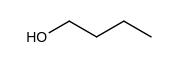
\includegraphics{smile-634b41a8e9c8b7bbba6ce3b1a8249d37b08577fa}\\
(2)\\
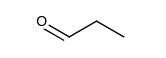
\includegraphics{smile-7df88a4bf8f88a43e1a13b7bcdfe93efbd0ab1f3}\\
(3) Aldehyde\\
(4) Carboxylic acid\\
(5) $\mathrm{CH}_{3} \mathrm{CH}_{2} \mathrm{CH}_{2} \mathrm{CH}_{2} \mathrm{COOH}$\\
(6) Ester\\
(7) $\mathrm{CH}_{3} \mathrm{CH}_{2} \mathrm{COOCH}_{2} \mathrm{CH}_{3}$\\
(8) Amine\\
(9)\\
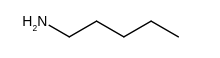
\includegraphics{smile-c1a62ec44c889f8991c4e8c00571ff3daf1c69a4}\\
11.9. Công thức cấu tạo của các hợp chất hữu cơ mạch hở có công thức phân tử $\mathrm{C}_{4} \mathrm{H}_{10} \mathrm{O}$ :\\
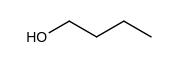
\includegraphics{smile-541c616d82f5fb3b6bc90a790b58ed3002fbd535}

(1)\\
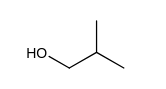
\includegraphics{smile-3aa3bf4fea8667f612d2cd71ff3329655532f031}

(2)\\
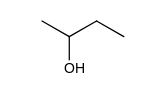
\includegraphics{smile-851d53338a0e757377fa90edda63c2906e8241fb}

(3)\\
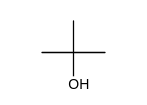
\includegraphics{smile-bb658aa506421f9fef30d09cf0df9a58904004bf}

(4)\\
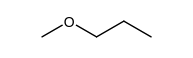
\includegraphics{smile-6e7ab1620e01424c09b8eeffcb3abda84e991995}

(5)\\
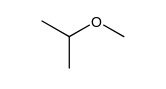
\includegraphics{smile-e01a6bfee9bd42c113f98a2c51781996ed8650b6}

(6)\\
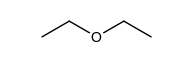
\includegraphics{smile-22c9be8c4ce3883b1a7db805dd1fd6b6d1722c8d}

(7)\\
a) Các chất là đồng phân nhóm chức alcohol: (1), (2), (3) và (4); các chất là đồng phân nhóm chức ether: (5), (6) và (7).\\
b) Các chất là đồng phân vị trí nhóm chức: (1) và (3); (5) và (7).\\
c) Các chất là đồng phân mạch carbon: (1) và (2); (5) và (6).\\
11.10. a) Các công thức (3) và (5) biểu diễn công thức cấu tạo của cùng một chất.\\
b) Các chất (2) và (4) biểu diễn công thức cấu tạo của hai đồng phân về vị trí nhóm chức.\\
11.11. a) Công thức phân tử của chất thứ 5 trong mỗi dãy đồng đẳng:

Dãy 1: $\mathrm{C}_{5} \mathrm{H}_{10} \mathrm{O}$; Dãy 2: $\mathrm{C}_{6} \mathrm{H}_{11} \mathrm{~N}$; Dãy 3: $\mathrm{C}_{10} \mathrm{H}_{14}$.\\
b) Công thức chung của các dãy:

Dãy 1: $\mathrm{C}_{\mathrm{n}} \mathrm{H}_{2 \mathrm{n}} \mathrm{O}(\mathrm{n} \geq 1) ;$ Dãy 2: $\mathrm{C}_{\mathrm{n}} \mathrm{H}_{2 \mathrm{n}-1} \mathrm{~N}(\mathrm{n} \geq 2) ;$ Dãy 3: $\mathrm{C}_{\mathrm{n}} \mathrm{H}_{2 \mathrm{n}-6}(\mathrm{n} \geq 6)$.\\
11.12. Các hợp chất $\mathrm{CH}_{3} \mathrm{COOH}\left(\mathrm{C}_{2} \mathrm{H}_{4} \mathrm{O}_{2}\right), \mathrm{HOCH} \mathrm{CH}_{2} \mathrm{CHO}\left(\mathrm{C}_{3} \mathrm{H}_{6} \mathrm{O}_{2}\right)$ và $\mathrm{CH}_{3} \mathrm{CH}_{2} \mathrm{COOCH}_{3}\left(\mathrm{C}_{4} \mathrm{H}_{8} \mathrm{O}_{2}\right)$ không thuộc cùng một dãy đồng đẳng do chúng có nhóm chức khác nhau.\\
$\mathrm{CH}_{3} \mathrm{COOH}\left(\mathrm{C}_{2} \mathrm{H}_{4} \mathrm{O}_{2}\right), \mathrm{CH}_{3} \mathrm{CH}_{2} \mathrm{COOH}\left(\mathrm{C}_{3} \mathrm{H}_{6} \mathrm{O}_{2}\right)$ và $\mathrm{CH}_{3} \mathrm{CH}_{2} \mathrm{CH}_{2} \mathrm{COOH}$ ( $\mathrm{C}_{4} \mathrm{H}_{8} \mathrm{O}_{2}$ ); hoặc $\mathrm{HOCH} 2 \mathrm{CHO}\left(\mathrm{C}_{2} \mathrm{H}_{4} \mathrm{O}_{2}\right), \mathrm{HOCH}_{2} \mathrm{CH}_{2} \mathrm{CHO}\left(\mathrm{C}_{3} \mathrm{H}_{6} \mathrm{O}_{2}\right)$ và $\mathrm{HOCH}_{2} \mathrm{CH}_{2} \mathrm{CH}_{2} \mathrm{CHO}\left(\mathrm{C}_{4} \mathrm{H}_{8} \mathrm{O}_{2}\right)$; hoặc $\mathrm{HCOOCH}_{3}\left(\mathrm{C}_{2} \mathrm{H}_{4} \mathrm{O}_{2}\right), \mathrm{CH}_{3} \mathrm{COOCH}_{3} \left(\mathrm{C}_{3} \mathrm{H}_{6} \mathrm{O}_{2}\right)$ và $\mathrm{CH}_{3} \mathrm{CH}_{2} \mathrm{COOCH}_{3}\left(\mathrm{C}_{4} \mathrm{H}_{8} \mathrm{O}_{2}\right)$.\\
11.13. a) Các nguyên tố có mặt trong thành phần phân tử của $\mathrm{A}: \mathrm{C}, \mathrm{H}$ và O .\\
b) Theo đề bài: $\left(\mathrm{CH}_{2} \mathrm{O}\right)_{n}=60$ hay $30 \mathrm{n}=60$ suy ra $\mathrm{n}=2$. Vậy A có công thức phân tử $\mathrm{C}_{2} \mathrm{H}_{4} \mathrm{O}_{2}$.\\
c) Trên phổ $\mathbb{R}$ của A thấy có tín hiệu hấp thự ở $1715 \mathrm{~cm}^{-1}$, đồng thời cũng thấy một đám hấp thụ trong vùng $3400-2500 \mathrm{~cm}^{-1}$ cho thấy A là một carboxylic acid. Do đó, A có công thức cấu tạo là $\mathrm{CH}_{3} \mathrm{COOH}$.\\
11.14. a) Từ bài cho, ta có:

$$
\frac{\mathrm{n}_{\mathrm{C}}}{\mathrm{n}_{\mathrm{H}}}=\frac{85,7: 12}{14,3: 1}=\frac{1}{2}
$$

Vậy công thức thực nghiệm của X là $\mathrm{CH}_{2}$.\\
b) Theo bài ra: $\left(\mathrm{CH}_{2}\right)_{\mathrm{n}}=56$ hay $14 \mathrm{n}=56$ suy ra $\mathrm{n}=4$.

Vậy công thức phân tử của X là $\mathrm{C}_{4} \mathrm{H}_{8}$.\\
c) cl) Với X là hydrocarbon mạch thẳng:\\
c2) Với X là hydrocarbon mạch hở, phân nhárih:

\section*{BÀ 12}
12.1.B. 12.2.B. 12.3.B. 12.4.A.\\
12.5. (c), (d). 12.6. C. 12.7. A.\\
12.8. B.\\
12.9. B.\\
12.10.A. 12.11.A. 12.12.A. 12.13.C. 12.14.B.\\
12.15. Do tính phản ứng chọn lọc của bromine nên sản phẩm chính là chất có nguyền tử H ở nguyên tử carbon có bậc cao nhất: $\left(\mathrm{CH}_{3}\right)_{2} \mathrm{CBrCH}_{2} \mathrm{CH}_{3}$.\\
12.16. $\mathrm{CH}_{2}=\mathrm{C}\left(\mathrm{CH}_{3}\right) \mathrm{CH}_{2} \mathrm{CH}_{3},\left(\mathrm{CH}_{3}\right)_{2} \mathrm{C}=\mathrm{CHCH}_{3},\left(\mathrm{CH}_{3}\right)_{2} \mathrm{CHCH}=\mathrm{CH}_{2}$.\\
12.17. a) Dầu nhẹ hơn nước, không tan trong nước, bị loang ra nên che phủ bề mặt biến làm giảm khả năng hoà tan của oxygen trong không khí vào trong nước biển, làm cho các sinh vật biển bị chết.\\
b) - Dừng các phao để gom dầu; việc dùng vật liệu hấp phụ dầu hiện đang nghiên cứu triến khai.

\begin{itemize}
  \item Hút dầu vào các bể chưa (lẫn nước biển).
  \item Chiết tách để loại bỏ nước, thu lấy dầu.\\
12.18*. Phưong án 1. Khai thác như khai thác than: đào mỏ; lấy các cục băng cháy, làm tan chảy thu lấy khí methane.
\end{itemize}

Phương án 2. Như kĩ thuật hiện đại khai thác sulfur: làm tan chảy băng cháy dưới lòng đất, thu khí bay lên.\\
12.19. Nếu chỉ dùng một loại hydrocarbon thì nhiệt giải phóng ra không đủ để khởi động động co. Và việc lưu trữ để đủ lượng xăng cho ô tô, xe máy sẽ khó khăn hơn (bình rất to hoặc phải là bình chịu áp suất cạo).\\
12.20. a) Tính lượng nhiệt toả ra khi đốt cháy 1 gam chất.

\begin{center}
\begin{tabular}{|l|l|l|l|l|l|}
\hline
Chat & Nhiet lurging (kd mol ) & Nhiét lumng/gan ( $\mathrm{K}^{-1}$ mol $\mathrm{g}^{-1}$ ) & Chát & Nhief lurnig (Id mol ) & Nhief lurong/gam ( $\mathrm{kl} \mathrm{mol}^{-1} \mathrm{~g}^{-1}$ ) \\
\hline
methane & 783 & 48,94 & propane & 2220 & 50,45 \\
\hline
ethane & 1570 & 52,33 & butane & 2875 & 46,57 \\
\hline
\end{tabular}
\end{center}

Như vậy, khi đốt cháy 1 gam mỗi chật trên, ethane sẽ sinh ra lượng nhiệt lớn nhất.\\
b) Từ kết quả phần a), ta thấy khối lượng chất cần đốt cháy ít nhất là ethane.\\
12.21. Trong 1 lít khí gas có 0,4 lít propane (số $\mathrm{mol}=0,0161 \mathrm{~mol}$ ) và 0,6 lít butane (số $\mathrm{mol}=0,0242$ ).\\
Lượng nhiệt toả ra tương ứng:\\
$0,0161.2220+0,0242.2875=35,742+69,575=105,317(\mathrm{~kJ})$.\\
12.22. - Làm thoáng không khí trong phòng bằng cách mở cửa.\\
-- Không được bật các thiết bị điện như quạt, đèn,...

\begin{itemize}
  \item Kiểm tra khoá bình gas, khoá lại nếu do quên chưa khoá.
  \item Báo cho nhà cung cấp gas để sửa chữa, thay thế nếu do van bị hỏng hoặc ống dẫn gas bị hở (do lâu ngày nên bị nứt, do chuột cắn,...).\\
12.23. Do các phương tiện giao thông đốt cháy nhiên liệu sinh ra nhiều khí carbon dioxide, các nitrogen oxide, carbon monoxide và các hạt bụi mịn do xăng, dầu cháy không hoàn toàn.
\end{itemize}

\section*{BÀI 13}
13.1. D.\\
13.2. C.\\
13.3. A. Các chất (1), (2) và (5) có đồng phân hình học.\\
13.4. B.\\
13.5. A. Phân tữ các alkene không hoặc rất ít phân cực, nên không tan trong nước và các dung môi phân cực mạnh.\\
13.6. A. Công thức thực nghiệm của X là $\mathrm{CH}_{2}$.\\
$\mathrm{M}_{\mathrm{X}}=42 \mathrm{~g} \mathrm{~mol}^{-1}$. Công thức phân tử của X là $\mathrm{C}_{3} \mathrm{H}_{6}$.\\
Vỉ X mạch hở, công thức phân tử dạng $\mathrm{C}_{\mathrm{n}} \mathrm{H}_{2 \mathrm{n}}$ chứng tỏ X là alkene.\\
Công thức cấu tạo phù hợp với X là $\mathrm{CH}_{2}=\mathrm{CHCH}_{3}$.\\
13.7.C.\\
13.8. A.\\
13.9. A. Alkene phản ứng với dung dịch $\mathrm{KMnO}_{4}$ tạo được hai nhóm OH tại hai nguyên tử carbon của liên kết đôi $\mathrm{C}=\mathrm{C}$.\\
13.10. D. Ở ống nghiệm (1) có kết tủa màu vàng nhạt là $\mathrm{AgC} \equiv \mathrm{CAg}$.

Ớ ống nghiệm (2) màu của nước bromine nhạt dần do $\mathrm{Br}_{2}$ phản ứng với ethylene (có thể có acetylene).\\
Ở ống nghiệm (2): sản phẩm tạo thành là $\mathrm{BrCH}_{2} \mathrm{CH}_{2} \mathrm{Br}$ (và có thể có $\mathrm{Br}_{2} \mathrm{CHCHBr}_{2}$ ) không tan trong nước và nặng hơn nước nên tách thành lớp dưới lớp nước bromine.\\
13.11. B.\\
13.12. D.\\
13.13. C.\\
13.14. Công thức cấu tạo và tên của các alkene có công thức phân tử $\mathrm{C}_{5} \mathrm{H}_{10}$ :\\
$\mathrm{CH}_{2}=\mathrm{CHCH}_{2} \mathrm{CH}_{2} \mathrm{CH}_{3}$ : pent-1-ene; $\mathrm{CH}_{2}=\mathrm{C}\left(\mathrm{CH}_{3}\right) \mathrm{CH}_{2} \mathrm{CH}_{3}$ : 2-methylbut-1-ene; $\mathrm{CH}_{2}=\mathrm{CHCH}\left(\mathrm{CH}_{3}\right) \mathrm{CH}_{3}$ : 3-methylbut-1-ene; $\mathrm{CH}_{3} \mathrm{CH}=\mathrm{CHCH}_{2} \mathrm{CH}_{3}$; pent-2-ene $\mathrm{CH}_{3} \mathrm{CH}=\mathrm{C}\left(\mathrm{CH}_{3}\right) \mathrm{CH}_{3}$ : 2-methylbut-2-ene.\\
Tên đầy đủ của các đồng phân hình học:\\
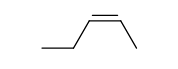
\includegraphics{smile-1b0d9c10054542f7ba5d2e07ccb057f16c5d35ba}

trans-pent-2-ene\\
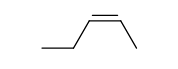
\includegraphics{smile-af3f7c560de951f64cdb6e62e88836c48bbb6fef}

cis-pent-2-ene\\
13.15. Dùng acetylene thuận lợi về kĩ thuật, do được điều chế trực tiếp từ chất rắn ( $\mathrm{CaC}_{2}$ ) mà việc bảo quản chất rắn (đất đèn) dễ dàng, it tốn diện tích. Nếu dùng trực tiếp các chất khí (ví dụ khí ethylene hoặc acetylene) sẽ gặp khó khăn do cần dùng bình nén khí dung tích lớn. Ví dụ: 1 kg đất đèn (kích thước bằng nắm tay) chứa $80 \%$ calcium carbide có ( 800 gam $\mathrm{CaC}_{2}$ ) có thể sinh ra $12,5 \mathrm{~mol}$ khí acetylene với thể tích 310 lít khí ở điều kiện chuẩn.\\
13.16*. Nguyên nhân là do việc điều chế acetylene giá thành cao hon.

Ethylene là sản phẩm phụ của quá trình hoá dầu (của quá trình cracking alkane) với lượng khí rất lớn. Nếu không tận dụng lượng khí này thì sẽ phải bỏ đi hoặc đốt cháy gây ô nhiễm môi trường.\\
13.17. Phản ứng oxi hoá làm phân cắt liên kết pi ( $\pi$ ) trong liên kết đôi $\mathrm{C}=\mathrm{C}$ của phân tử ethylene và trong liên kết ba $\mathrm{C}=\mathrm{C}$ của phân tử acetylene. Do liên kết ba $\mathrm{C} \equiv \mathrm{C}$ bền hơn liên kết đôi $\mathrm{C}=\mathrm{C}$ nên khó bị phân cắt hơn.\\
13.18. Công thức thực nghiệm của chất là $\mathrm{CH}_{2}$.\\
$\mathrm{M}_{\mathrm{X}}=70$ gam $\mathrm{mol}^{-1}$. Vậy công thức phân tử của chất là $\mathrm{C}_{5} \mathrm{H}_{10}$.\\
Công thức phân tử của các hydrocarbon mạch hở có dạng $\mathrm{C}_{\mathrm{n}} \mathrm{H}_{2 \mathrm{n}}$ chứng tỏ chúng là alkene. Công thức cấu tạo của các alkene $\mathrm{C}_{5} \mathrm{H}_{10}$ là:\\
$\mathrm{CH}_{2}=\mathrm{CHCH}_{2} \mathrm{CH}_{2} \mathrm{CH}_{3} ; \mathrm{CH}_{2}=\mathrm{C}\left(\mathrm{CH}_{3}\right) \mathrm{CH}_{2} \mathrm{CH}_{3} ; \mathrm{CH}_{2}=\mathrm{CHCH}\left(\mathrm{CH}_{3}\right) \mathrm{CH}_{3} ;$\\
$\mathrm{CH}_{3} \mathrm{CH}=\mathrm{CHCH}_{2} \mathrm{CH}_{3} ; \mathrm{CH}_{3} \mathrm{CH}=\mathrm{C}\left(\mathrm{CH}_{3}\right) \mathrm{CH}_{3}$.

\section*{BÀ 14}
14.1. B.\\
14.2. B.\\
14.3. A. Công thức phân tử của Y là $\mathrm{C}_{8} \mathrm{H}_{8}$.

Vì Y là arene nên phân tử có vòng benzene.\\
Vậy Y có công thức cấu tạo $\mathrm{C}_{6} \mathrm{H}_{5} \mathrm{C}_{2} \mathrm{H}_{3}$ hay $\mathrm{C}_{6} \mathrm{H}_{5} \mathrm{CH}=\mathrm{CH}_{2}$.\\
14.4. D.\\
14.5. B. Các chất (1), (4), (5) và (6) là đồng phân cấu tạo của nhau.\\
14.6. C.\\
14.7. A.\\
14.8. A. Là hợp chất phân tử có một nhánh liên kết với vòng benzene.\\
14.9. C. Chí phenylacetylene phản úng được với dung dịch $\mathrm{AgNO}_{3} / \mathrm{NH}_{3}$ tạo ra kết tủa.\\
14.10. A. Khi đun nóng với dung dịch $\mathrm{KMnO}_{4}$ trong môi trường $\mathrm{H}_{2} \mathrm{SO}_{4}$ tạo hợp chất hữu cơ đơn chức $Y$ chứng tỏ phân tử $X$ có một nhánh ở vòng benzene, nên có công thức cấu tạo là $\mathrm{C}_{6} \mathrm{H}_{5} \mathrm{CH}_{2} \mathrm{CH}_{3}$.\\
14.11. D. Đã xảy ra phản ứng thế nguyên tử H của vòng benzene bằng nhóm $\mathrm{NO}_{2}$.\\
14.12. A.\\
14.14.\\
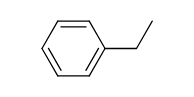
\includegraphics{smile-9d26afc9e977b2dc09be45dae9a19814d59a97b3}\\
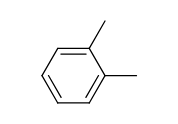
\includegraphics{smile-1ec89c6a500ab8ff5c996972cd16e5b23d040578}\\
14.13. B.\\
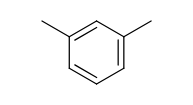
\includegraphics{smile-d148bf3b30bbcf35406876ca0731f9ff3cc75336}\\
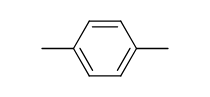
\includegraphics{smile-cb2929419649cae8e79faa0ae0b2e5e67391466b}\\
14.15. Cách 1. Cho từng chất toluene, styrene, benzene vào bình cầu đựng dung dịch $\mathrm{KMnO}_{4}$, khuấy nhẹ ở điều kiện thường. Khi đó, styrene phản ứng làm nhạt màu dung dịch $\mathrm{KMnO}_{4}$. Đun nóng và khuấy hỗn hợp trong hai bình còn lại: toluene là chất làm mât màu/ nhạt màu dung dịch $\mathrm{KMnO}_{4}$; benzene thì không có hiện tượng đó.\\
Cách 2. Cho từng chất toluene, styrene, benzene vào ống nghiệm đựng dung dịch $\mathrm{Br}_{2} / \mathrm{CCl}_{4}$, lắc nhẹ. Styrene phản úng làm nhạt màu bromine; đặt mẩu giấy quỳ ẩm lên miệng hai ống nghiệm còn lại và chiếu ánh sáng tử ngoại vào hai ống nghiệm này: toluene là chất làm quỳ tím ẩm chuyển thành màu đỏ do có phản ứng thế tạo thành $\mathrm{C}_{6} \mathrm{H}_{5} \mathrm{CH}_{2} \mathrm{Br}$ và HBr bay ra; benzene không phản ứng trong điều kiện này.\\
14.16. Công thức thực nghiệm của X là $\mathrm{C}_{4} \mathrm{H}_{3}$.\\
$\mathrm{M}_{\mathrm{x}}=102 \mathrm{~g} \mathrm{~mol}^{-1}$. Công thức phân tử của X là $\mathrm{C}_{8} \mathrm{H}_{6}$.\\
Vì X có khả năng phản ứng với bromine khi có xúc tác $\mathrm{FeBr}_{3}$, chứng tỏ phân tử\\
X có vòng benzene. Vậy công thức cấu tạo phù hợp với X là:\\
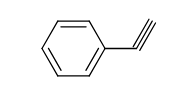
\includegraphics{smile-5dee41d9c7ba97fe503d8c48a838edde71372713}

\section*{BÀI 15}
15.1.C.\\
15.2. A.\\
15.3. (b), (c), (d).\\
15.4. (a), (c).\\
15.5. D.\\
(2) khí\\
(3) gây hại\\
(4) nhà kính\\
15.6. (1) chlorodifluoromethane\\
15.7*. Điều chế halothane từ 2-chloro-1,1,1-trifluoroethane bằng phản ứng thế bromine.

$$
\mathrm{CF}_{3} \mathrm{CH}_{2} \mathrm{Cl}+\mathrm{Br}_{2} \rightarrow \mathrm{CF}_{3} \mathrm{CHBrCl}+\mathrm{HBr}
$$

15.8. a) A là dẫn xuất monochloro của alkylbenzene nên công thức phân tử của A có dạng $\mathrm{C}_{\mathrm{n}} \mathrm{H}_{2 \mathrm{n}-7} \mathrm{Cl}$.\\
$12 \mathrm{n}+2 \mathrm{n}-7+35,5=126,5 \Rightarrow \mathrm{n}=7 \Rightarrow$ Công thức phân tử của A là $\mathrm{C}_{7} \mathrm{H}_{7} \mathrm{Cl}$.\\
Các công thức cấu tạo có thể có của A :\\
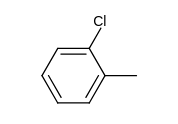
\includegraphics{smile-2bdfa513112a1638a51d15af02274ada0909ff1f}

(1)\\
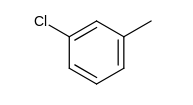
\includegraphics{smile-dc5b33cb5b38b9fea4399a474cbc52574ef5d0fd}

(2)\\
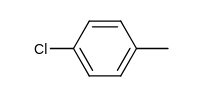
\includegraphics{smile-e51d8ce81a1b169367232dc94837c091823d4bb4}

(3)\\
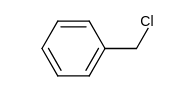
\includegraphics{smile-d76584a686c8324284ff8b4f33fb5036eb5184e2}

(4)\\
b) A có phản ứng thử phân khi đun nóng với dung dịch NaOH nên công thức cấu tạo phù hợp của $\mathbb{A}$ là (4).\\
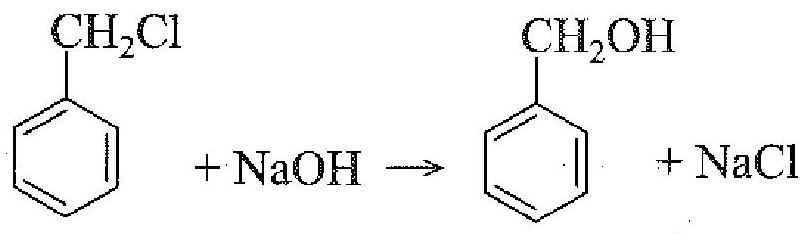
\includegraphics[max width=\textwidth, center]{2025_10_23_052d3249fabea90c1e95g-23}\\
c) Phương trình hoá học của phản ứng điều chế trực tiếp $\mathbf{A}$ từ $\mathbf{B}$ :\\
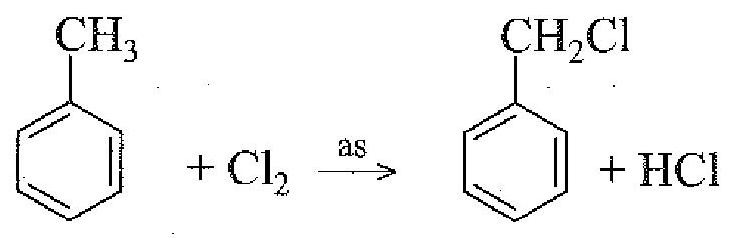
\includegraphics[max width=\textwidth, center]{2025_10_23_052d3249fabea90c1e95g-23(2)}\\
15.9*. a)\\
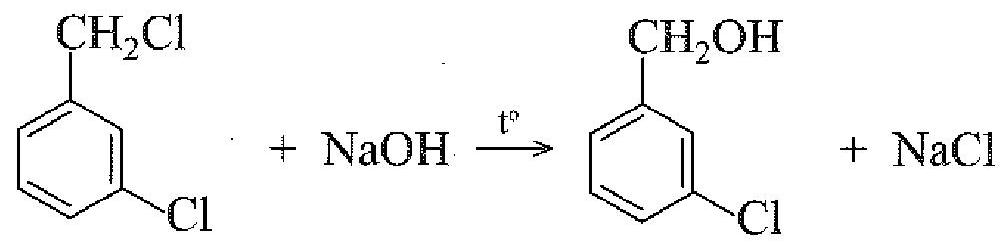
\includegraphics[max width=\textwidth, center]{2025_10_23_052d3249fabea90c1e95g-23(1)}\\
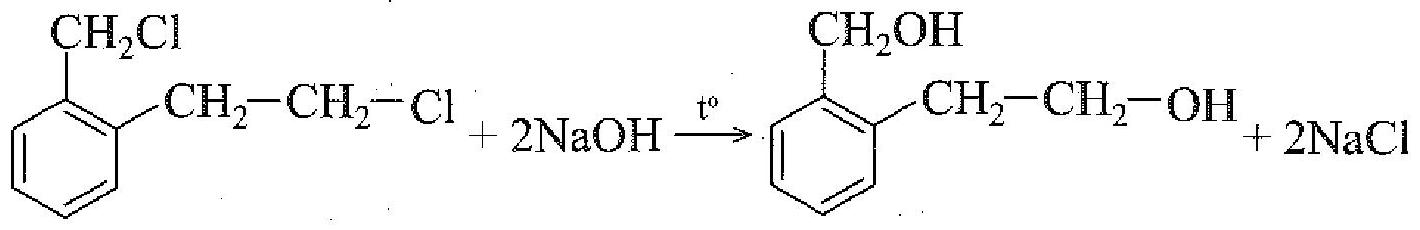
\includegraphics[max width=\textwidth, center]{2025_10_23_052d3249fabea90c1e95g-23(3)}\\
b) Khả năng tham gia phản ứng thế:\\
$\mathrm{R}-\mathrm{CH}=\mathrm{CH}-\mathrm{CH}_{2} \mathrm{Cl}, \mathrm{R}-\mathrm{CH}_{2} \mathrm{Cl}>\mathrm{R}-\mathrm{C}_{6} \mathrm{H}_{4} \mathrm{Cl}$.\\
15.10*. a) Do 2,4-D kém tan trong nước, tan tốt trong ethanol nên đầu tiên người ta hoà tan trong cồn $50^{\circ}$, sau đó thêm nước cho đủ 100 mL .\\
b) Nồng độ dung dịch 2,4-D là: $100: 100=1\left(\mathrm{mg} \mathrm{mL}^{-1}\right)$.

\section*{BÀI 16}
16.1. A.\\
16.2. A. 16.3. B.\\
16.4. D. Các phát biểu đúng là (a), (b), (d).\\
16.5. (a), (b), (d).\\
16.6. B.\\
16.7. D.\\
16.8. C.\\
16.9. a - 1,$4 ; \mathrm{b}-3,4 ; \mathrm{c}-1,5 ; \mathrm{d}-2,4$.\\
16.10.\\
(1) $\mathrm{CH}_{3}-\mathrm{CH}_{2}-\mathrm{O}-\mathrm{CH}_{3}$\\
(2) $\mathrm{CH}_{3}-\mathrm{CH}_{2}-\mathrm{CH}_{2}-\mathrm{OH}$\\
(3) $\mathrm{CH}_{3}-\mathrm{CH}(\mathrm{OH})-\mathrm{CH}_{3}$\\
(4) propan-1-ol\\
(5) propan-2-ol\\
(6) không xảy ra\\
(7) tạo ra $\mathrm{H}_{2}$\\
(8) tao ra $\mathrm{H}_{2}$\\
(9) không xảy ra\\
(10) tạo ra aldehyde $\mathrm{CH}_{3}-\mathrm{CH}_{2}-\mathrm{CHO}$\\
(11) tạo ra ketone $\mathrm{CH}_{3}-\mathrm{CO}-\mathrm{CH}_{3}$.\\
16.11. a) glycerol\\
b) dung dịch có màu xanh đậm\\
c) (1) 3;\\
(2) $\mathrm{CH}_{3}-\mathrm{O}-\mathrm{CH}_{3}$,\\
$\mathrm{C}_{2} \mathrm{H}_{5}-\mathrm{O}-\mathrm{C}_{2} \mathrm{H}_{5}, \mathrm{CH}_{3}-\mathrm{O}-\mathrm{C}_{2} \mathrm{H}_{5}$\\
d) 2 .\\
16.12*. a) Từ phần trăm nguyên tố của X , xác định được công thức đơn giản nhất của X là $\mathrm{C}_{4} \mathrm{H}_{10} \mathrm{O}$. Từ phổ MS của X cho thấy X có phân tử khối bằng 74 . $74 \mathrm{n}=74 \Rightarrow \mathrm{n}=1$. Vậy công thức phân tử của X là $\mathrm{C}_{4} \mathrm{H}_{10} \mathrm{O}$.\\
b) Do trên phổ IR của X có tín hiệu ở vùng $3650-3200 \mathrm{~cm}^{-1}$ nên X là một alcohol.\\
Công thức cấu tạo có thể có của $\mathbf{X}$ là: $\mathrm{CH}_{3}-\mathrm{CH}_{2}-\mathrm{CH}_{2}-\mathrm{CH}_{2}-\mathrm{OH}$, $\mathrm{CH}_{3}-\mathrm{CH}(\mathrm{OH})-\mathrm{CH}_{2}-\mathrm{CH}_{3},\left(\mathrm{CH}_{3}\right)_{2} \mathrm{CH}-\mathrm{CH}_{2}-\mathrm{OH}$ và $\left(\mathrm{CH}_{3}\right)_{3} \mathrm{C}-\mathrm{OH}$.\\
c) Do oxi hoá X bằng CuO , đun nóng, thu được một aldehyde có mạch carbon phân nhánh nên X có công thức cấu tạo là $\left(\mathrm{CH}_{3}\right)_{2} \mathrm{CH}-\mathrm{CH}_{2}-\mathrm{OH}$ và tên gọi là 2-methylpropan-1-ol.\\
16.13*. Số $\mathrm{mol} \mathrm{H}_{2}$ là: $0,6197: 24,790 \approx 0,025(\mathrm{~mol})$.

Số mol xylitol là: $1,52: 152=0,01(\mathrm{~mol})$.\\
Xylitol có công thức phân tử dạng $\mathrm{C}_{\mathrm{n}} \mathrm{H}_{2 \mathrm{n}+2} \mathrm{O}_{5}$, giữa các nguyên tử không có liên kết $\pi$, nên chỉ có nhóm OH tác dụng với Na tạo $\mathrm{H}_{2}$.\\
Đặt số nhóm OH trong phân tử xylitol là x , xylitol có dạng $\mathrm{R}(\mathrm{OH})_{\mathrm{x}}$

$$
\begin{aligned}
& 2 \mathrm{R}(\mathrm{OH})_{\mathrm{x}}+2 \mathrm{xNa} \longrightarrow 2 \mathrm{R}(\mathrm{ONa})_{\mathrm{x}}+\mathrm{xH}_{2} \\
& \quad 0,01 \\
& \Rightarrow \mathrm{x}=5
\end{aligned}
$$

Một nguyên tử C chỉ liên kết tối đa với một nhóm -OH , do đó, công thức cấu tạo cúa xylitol là $\mathrm{CH}_{2} \mathrm{OH}[\mathrm{CHOH}]_{3} \mathrm{CH}_{2} \mathrm{OH}$.\\
16.14. a) Quá trình lên men: $\left(\mathrm{C}_{6} \mathrm{H}_{10} \mathrm{O}_{5}\right)_{\mathrm{n}} \xrightarrow[\mathrm{H}_{2} \mathrm{O}]{\text { enzyme }} \mathrm{C}_{6} \mathrm{H}_{12} \mathrm{O}_{6} \xrightarrow[-\mathrm{CO}_{2}]{\text { enzyme }} \mathrm{C}_{2} \mathrm{H}_{5} \mathrm{OH}$

Từ quá trình trên, tính được khối lượng ethyl alcohol là:

$$
\frac{1000.38}{100.262} \cdot 2.46 \cdot \frac{81}{100}=174,8(\mathrm{~kg})
$$

b) Thể tích của ethyl alcohol là: $174,8: 0,8=218,5(\mathrm{~L})$.

Thể tích xăng E5 sau khi pha trộn là: $218,5.100: 5=4370(\mathrm{~L})$.\\
16.15*.\\
a)\\
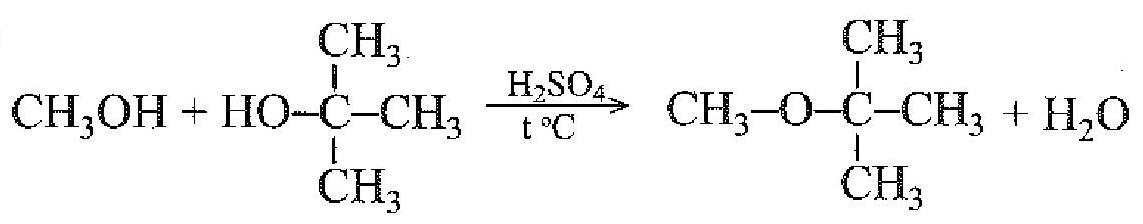
\includegraphics[max width=\textwidth, center]{2025_10_23_052d3249fabea90c1e95g-25}

Phương pháp điều chế MTBE từ hai alcohol tương ứng không phù hợp để tổng hợp MTBE trong công nghiệp vì sẽ thu được hỗn hợp ether.\\
b) $\mathrm{CH}_{3} \mathrm{OH}+\mathrm{CH}_{2}=\stackrel{\mathrm{CH}_{3}}{\mathrm{C}}-\mathrm{CH}_{3} \xrightarrow[t^{\circ} \mathrm{C}]{\mathrm{H}_{2} \mathrm{SO}_{4}}$\\
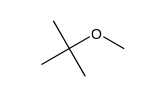
\includegraphics{smile-ce3e0712c8b69812f5f7396086f10f6812bf7cf3}

\section*{BÀI 17}
17.1. A.\\
17.2. A.\\
17.3. A.\\
17.4. C.\\
17.5. D.\\
17.6*. B.\\
17.7.B.\\
17.8*. b) Phân tử picric acid dễ gây cháy, nổ mạnh nên để an toàn, thường bảo quản picric acid trong lọ dưới một lớp nước. Mặt khác, picric acid có tính acid mạnh, phản ứng với kim loại toả nhiệt, tạo muối picrate cũng dễ gây cháy nổ.\\
17.9. a) Dặt công thức của A là $\mathrm{C}_{\mathrm{x}} \mathrm{H}_{\mathrm{y}} \mathrm{O}$.

Khối lượng mol của A là: $\frac{16}{14,81} \cdot 100=108\left(\mathrm{~g} \mathrm{~mol}^{-1}\right)$.

$$
x=\frac{77,78}{12 \cdot 100} \cdot 108=7 ; \quad y=\frac{7,41}{100} \cdot 108=8
$$

Vậy công thức phân tữ của A là $\mathrm{C}_{7} \mathrm{H}_{8} \mathrm{O}$.\\
b) Thí nghiệm chứng tỏ A không tan trong nước, A tác dụng với NaOH , vậy A là phenol. Công thức cấu tạo của A là một trong số ba công thức cấu tạo sau:\\
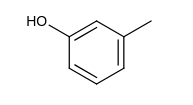
\includegraphics{smile-d2ed27f42107b6411d7f3ea6b37390536c5e8021}\\
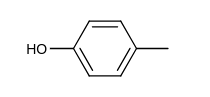
\includegraphics{smile-0f8c0f725ad0cc3e18493b94463c9121d9a4e31b}\\
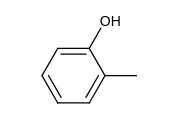
\includegraphics{smile-c2385a39a7d9cf8c3714f0eee93542a49a97d0ef}\\
c) Chất $\mathbf{B}$ là một trong số các đồng phân (có vòng benzene) của\\
A. Chất B không tác dựng với Na , không tác dụng với NaOH nên B là methyl phenyl ether:\\
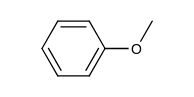
\includegraphics{smile-59ee17f34366a7a1401b21c599fe4d6f7f038f33}\\
$17.10^{*}$. a) Công thức phân tử của vanillin: $\mathrm{C}_{8} \mathrm{H}_{8} \mathrm{O}_{3}$.\\
b) Vanillin khó tan trong nước, dễ tan trong ethanol, tan trong dung dịch kiềm.\\
c) Số mol NaOH là: $\quad \frac{7,82.0,1}{1000}=7,82 \cdot 10^{-4}(\mathrm{~mol})$

$$
\mathrm{HOC}_{6} \mathrm{H}_{3}\left(\mathrm{OCH}_{3}\right)(\mathrm{CHO})+\mathrm{NaOH} \rightarrow \mathrm{NaOC}_{6} \mathrm{H}_{3}\left(\mathrm{OCH}_{3}\right)(\mathrm{CHO})+\mathrm{H}_{2} \mathrm{O}
$$

Số mol vanillin $\mathrm{C}_{8} \mathrm{H}_{8} \mathrm{O}_{3}$ bằng số mol NaOH và bằng $7,82 \cdot 10^{-4} \mathrm{~mol}$.\\
Phần trăm khối lượng vanillin trong mẫu trên là: $\frac{7,82 \cdot 10^{-4} \cdot 152}{0,12} \cdot 100 \%=99,05 \%$.\\
Mẫu vanillin trên đủ tiêu chuẩn dùng trong công nghiệp sản xuất dược phẩm và thực phẩm.\\
17.11. a)\\
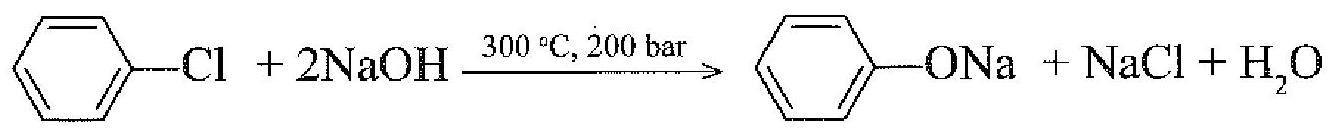
\includegraphics[max width=\textwidth, center]{2025_10_23_052d3249fabea90c1e95g-26}\\
b) Sơ đồ điều chế phenol từ benzene và các chất vô co.\\
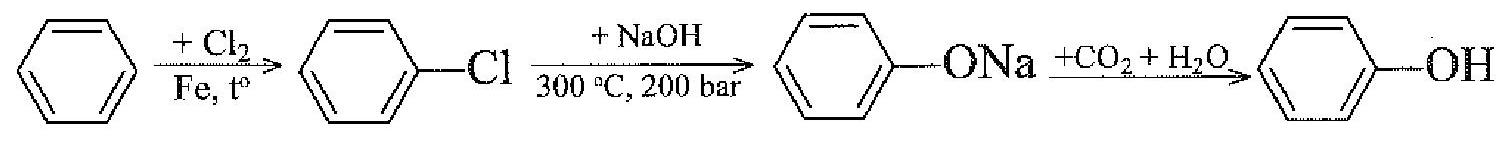
\includegraphics[max width=\textwidth, center]{2025_10_23_052d3249fabea90c1e95g-26(1)}\\
c) Khối lượng benzene cần thiết là: $\frac{9,4.78 .100}{94.42}=18,57(\mathrm{~kg})$.

\section*{BÀl 18}
18.1.D. 18.2. $a-4 ; b-1 ; c-3, d-2$.\\
18.3.C. 18.4.B. 18.5.A. 18.6.D.\\
18.7. D. 18.8. D. 18.9. C. 18.10. A. 18.11. D\\
18.12. B. 18.13. D. 18.14. C. 18.15. A.\\
18.16. (1) liên kết $\pi$; (2) lớn hơn; (3) electron; (4) liên kết $\mathrm{C}=\mathrm{O}$; (5) âm; (6) dương.\\
18.17. (1) $\mathrm{CH}_{3} \mathrm{CH}_{3}+\mathrm{Cl}_{2} \xrightarrow{\text { as }} \mathrm{CH}_{3} \mathrm{CH}_{2} \mathrm{Cl}+\mathrm{HCl}$\\
(2) $\mathrm{CH}_{3} \mathrm{CH}_{2} \mathrm{Cl}+\mathrm{NaOH} \xrightarrow{\mathrm{t}^{\circ}} \mathrm{CH}_{3} \mathrm{CH}_{2} \mathrm{OH}+\mathrm{NaCl}$\\
(3) $\mathrm{CH}_{3} \mathrm{CH}_{2} \mathrm{OH}+\mathrm{CuO} \xrightarrow{t^{\circ}} \mathrm{CH}_{3} \mathrm{CHO}+\mathrm{Cu}+\mathrm{H}_{2} \mathrm{O}$\\
(4) $\mathrm{CH}_{3} \mathrm{CHO}+\mathrm{Br}_{2}+\mathrm{H}_{2} \mathrm{O} \longrightarrow \mathrm{CH}_{3} \mathrm{COOH}+2 \mathrm{HBr}$\\
18.18. (1) butan-2-one (2) butanal (3) 2-methylpropanal\\
(4) $\mathrm{CH}_{3} \mathrm{CH}(\mathrm{OH}) \mathrm{CH}_{2} \mathrm{CH}_{3}$ (5) $\mathrm{CH}_{3} \mathrm{CH}_{2} \mathrm{CH}_{2} \mathrm{CH}_{2} \mathrm{OH}$ (6) $\left(\mathrm{CH}_{3}\right)_{2} \mathrm{CHCH}_{2} \mathrm{OH}$\\
(7) Không phản ứng (8) $\mathrm{CH}_{3} \mathrm{CH}_{2} \mathrm{CH}_{2} \mathrm{COOH}$ (9) $\left(\mathrm{CH}_{3}\right)_{2} \mathrm{CHCOOH}$\\
(10) Không phản ứng (11) $\mathrm{CH}_{3} \mathrm{CH}_{2} \mathrm{CH}_{2} \mathrm{COONH}_{4}$\\
(12) $\left(\mathrm{CH}_{3}\right)_{2} \mathrm{CHCOONH}_{4}$ (13) Không phản ứng\\
(14) $\mathrm{CH}_{3} \mathrm{CH}_{2} \mathrm{CH}_{2} \mathrm{COONa}$ (15) $\left(\mathrm{CH}_{3}\right)_{2} \mathrm{CHCOONa}$.\\
18.19. a) $\mathrm{A}: \mathrm{CH}_{3} \mathrm{CHBrCH}_{3} ; \mathrm{B}: \mathrm{CH}_{3} \mathrm{CH}(\mathrm{OH}) \mathrm{CH}_{3} ; \mathrm{C}: \mathrm{CH}_{3} \mathrm{COCH}_{3}$.\\
b) Chất $\mathbb{B}$ có tín hiệu đặc trưng ở vùng $3650-3200 \mathrm{~cm}^{-1}$.

Chất C có tín hiệu đặc trưng ở vùng $1740-1670 \mathrm{~cm}^{-1}$.\\
18.20. Do trong khói của bếp có chưa formaldehyde (HCHO), chất này có khả năng diệt trùng, chống mối mọt nên các vật dụng rổ, rá, nong, nia,... bền hơn.\\
18.21. a) Ta có $\% \mathrm{~m}_{\mathrm{O}}=22,22 \%$

Công thức đơn giản nhất của X là $\mathrm{C}_{4} \mathrm{H}_{8} \mathrm{O}$.\\
Gọi công thức phân tử của X là $\left(\mathrm{C}_{4} \mathrm{H}_{8} \mathrm{O}\right)_{\mathrm{n}}$

$$
\Rightarrow M_{x}=(4.12+8+16) n=72 n=72 \Rightarrow n=1
$$

Vậy công thức phân tử của X là $\mathrm{C}_{4} \mathrm{H}_{8} \mathrm{O}$.\\
b) X không tác dụng được với dung dịch $\mathrm{AgNO}_{3}$ trong $\mathrm{NH}_{3}$ nên X là ketone. Do X có phản ứng tạo iodoform nên phân tử của X có chứa nhóm $\mathrm{CH}_{3} \mathrm{CO}$. Vậy công thức cấu tạo của X là $\mathrm{CH}_{3} \mathrm{COCH}_{2} \mathrm{CH}_{3}$ (ethyl methyl ketone hay butanone).\\
18.22*. Trên phổ $\mathrm{IR}, \mathrm{A}$ và B có tín hiệu đặc trưng ở vùng $1740-1670 \mathrm{~cm}^{-1}$ nên A và B là hợp chất carbonyl.\\
C có tín hiệu đặc trưng ở vùng $3650-3200 \mathrm{~cm}^{-1}$ nên C là hợp chất alcohol.\\
A là aldehyde đơn chức nên phân tử A chỉ có 1 nguyên tữ oxygen. Vậy $\mathrm{A}, \mathbb{B}$ và C có cùng công thức phân tử $\mathrm{C}_{3} \mathrm{H}_{6} \mathrm{O}$.

Vi $\mathbb{A}$ là aldehyde và $\mathbb{B}$ là ketone nên $\mathbb{A}$ và $\mathbb{B}$ có công thức như sau:\\
A: $\mathrm{CH}_{3} \mathrm{CH}_{2} \mathrm{CHO}$ (propanal)\\
$\mathrm{B}: \mathrm{CH}_{3} \mathrm{COCH}_{3}$ (acetone hay propanone)\\
$\mathbb{C}$ là alcohol nên $\mathbb{C}$ có công thức là $\mathrm{CH}_{2}=\mathrm{CHCH}_{2} \mathrm{OH}$ (prop-2-en-1-ol hay allyl alcohol).\\
$18.23^{*}$. a) $\mathrm{m}_{\text {phenol }}=744,16 \mathrm{~kg} ; \mathrm{m}_{\text {acetone }}=459,16 \mathrm{~kg}$.\\
b) $\mathrm{m}_{\text {bisphenol A }}=722 \mathrm{~kg}$.\\
18.24*. a) Trong sản xuất gỗ công nghiệp, người ta sử dụng một lượng lớn keo dán, đó chính là nhựa poly(phenol-formaldehyde). Nhưa poly(phenolformaldehyde) được sản xuất từ formaldehyde và phenol. Do vậy trong keo dán thường có một lượng nhỏ formaldehyde.\\
b) Lượng formaldehyde có trong 1 g gỗ là: $\frac{0,03}{300}=10^{-4}(\mu \mathrm{~g})$

Lượng formaldehyde có trong 800 kg (hay $1 \mathrm{~m}^{3}$ ) gỗ là:

$$
10^{-4} \cdot 800 \cdot 10^{3}=80(\mu \mathrm{~g})
$$

Như vậy, lô gỗ đạt tiêu chuẩn xuất khẩu sang châu Âu.\\
18.25*. a) Từ thành phần nguyên tố, xác định được công thức đơn giản nhất của A là $\mathrm{C}_{9} \mathrm{H}_{8} \mathrm{O}$. Kết hợp với giá trị phân tử khối, xác định được công thức phân tứ của A là $\mathrm{C}_{9} \mathrm{H}_{8} \mathrm{O}$.

\begin{itemize}
  \item Trên phổ $\mathbb{R}$ của $\mathbf{A}$ có một tín hiệu đặc trưng ở $1746 \mathrm{~cm}^{-1}$ chứng tỏ A chứa nhóm $\mathrm{C}=\mathrm{O}$.
  \item A có phản ứng tráng bạc, chứng tỏ A là aldehyde.
  \item A làm mất màu dung dịch $\mathrm{Br}_{2} / \mathrm{CCl}_{4}$ chứng tó trong A chứa $\mathrm{C}=\mathrm{C}$.
  \item Khi bị oxi hoá bằng dung dịch $\mathrm{KMnO}_{4}$ nóng, thu đưọc benzoic acid, chứng tô A là dẫn xuất một lần thế của benzene.\\
Công thức cấu tạo của A là $\mathrm{C}_{6} \mathrm{H}_{5} \mathrm{CH}=\mathrm{CHCHO}$ (cinnamaldehyde).\\
b) Công thức của $\mathbf{A}$ là:\\
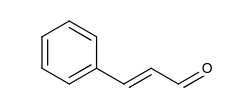
\includegraphics{smile-18406a036b1f8a4c5214b0b5cb02f93053ff2643}
\end{itemize}

\section*{BÀI 19}
\begin{center}
\begin{tabular}{llll}
19.1. C. & 19.2. D. & 19.3. C. & 19.4. D. \\
19.5. D. & 19.6. D. & 19.7. C. & 19.8. B. \\
19.9. A. & 19.10. D. & 19.11. C. & 19.12. C. \\
\end{tabular}
\end{center}

19.13. A.

Gọi công thức của X là RCOOH .\\
$2 \mathrm{RCOOH}+\mathrm{CaCO}_{3} \longrightarrow(\mathrm{RCOO})_{2} \mathrm{Ca}+\mathrm{CO}_{2} \uparrow+\mathrm{H}_{2} \mathrm{O}$\\
$\mathrm{n}_{\mathrm{x}}=(7,28-5,76): 19=0,08(\mathrm{~mol}) \Rightarrow \mathrm{M}_{\mathrm{x}}=5,76: 0,08=72\left(\mathrm{~g} \mathrm{~mol}^{-1}\right)$.\\
Vậy X có công thức là: $\mathrm{CH}_{2}=\mathrm{CHCOOH}$.\\
19.14. B.\\
19.15*. D.\\
19.16. - Điều chế formaldehyde từ methane:

$$
\begin{aligned}
& \mathrm{CH}_{4}+\mathrm{Cl}_{2} \xrightarrow{\text { as }} \mathrm{CH}_{3} \mathrm{Cl}+\mathrm{HCl} \\
& \mathrm{CH}_{3} \mathrm{Cl}+\mathrm{NaOH} \xrightarrow{\mathrm{t}^{\circ}} \mathrm{CH}_{3} \mathrm{OH}+\mathrm{NaCl} \\
& \mathrm{CH}_{3} \mathrm{OH}+\mathrm{CuO} \xrightarrow{\mathrm{t}^{\circ}} \mathrm{HCHO}+\mathrm{Cu}+\mathrm{H}_{2} \mathrm{O}
\end{aligned}
$$

\begin{itemize}
  \item Diều chế acetic acid từ methane:
\end{itemize}

Lấy $\mathrm{CH}_{3} \mathrm{OH}$ từ trên: $\mathrm{CH}_{3} \mathrm{OH}+\mathrm{CO} \xrightarrow{t^{\circ}, \mathrm{xt}} \mathrm{CH}_{3} \mathrm{COOH}$\\
Hoặc: $2 \mathrm{CH}_{4} \xrightarrow[\text { Làm lạnh nhanh }]{1500^{\circ} \mathrm{C}} \mathrm{C}_{2} \mathrm{H}_{2}+3 \mathrm{H}_{2}$\\
$\mathrm{C}_{2} \mathrm{H}_{2}+\mathrm{H}_{2} \mathrm{O} \xrightarrow{\mathrm{Hg}^{2+}, 80^{\circ} \mathrm{C}} \mathrm{CH}_{3} \mathrm{CHO}$\\
$\mathrm{CH}_{3} \mathrm{CHO}+2\left[\mathrm{Ag}\left(\mathrm{NH}_{3}\right)_{2}\right] \mathrm{OH} \longrightarrow \mathrm{CH}_{3} \mathrm{COONH}_{4}+3 \mathrm{NH}_{3}+2 \mathrm{Ag}+\mathrm{H}_{2} \mathrm{O}$\\
$\mathrm{CH}_{3} \mathrm{COONH}{ }_{4}+\mathrm{HCl} \rightarrow \mathrm{CH}_{3} \mathrm{COOH}+\mathrm{NH}_{4} \mathrm{Cl}$\\
19.17. Cách làm như vậy là đúng. Bạn Hiền đã dùng phương pháp kết tinh, dựa trên lí do cát không tan trong nước còn benzoic acid tan tốt trong nước nóng nhưng it tan trong nước lạnh.\\
Ngoài cách làm trên, có thể đun nóng hỗn hợp và ngưng tụ hơi benzoic acid bay lên thu được acid do benzoic acid thăng hoa.\\
19.18.\\
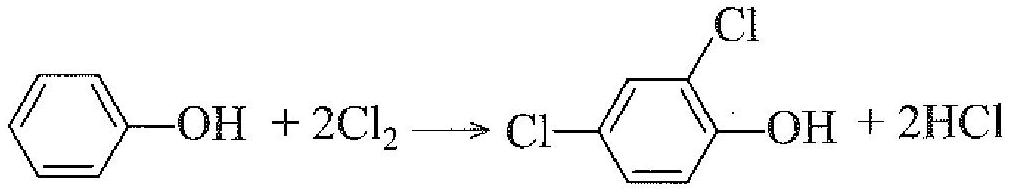
\includegraphics[max width=\textwidth, center]{2025_10_23_052d3249fabea90c1e95g-30(1)}\\
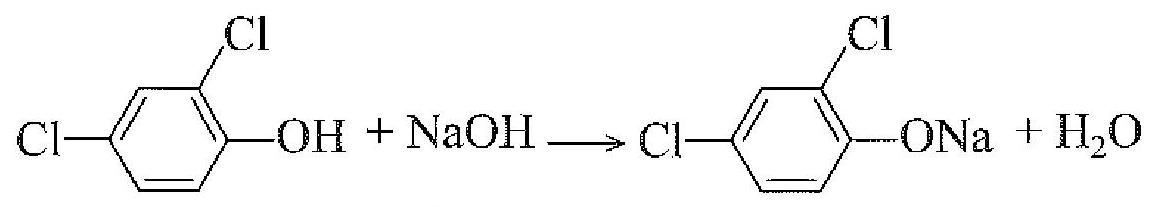
\includegraphics[max width=\textwidth, center]{2025_10_23_052d3249fabea90c1e95g-30}\\
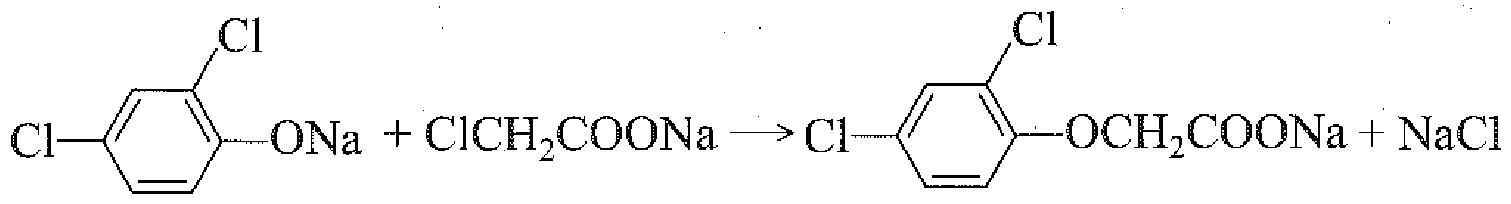
\includegraphics[max width=\textwidth, center]{2025_10_23_052d3249fabea90c1e95g-30(2)}\\
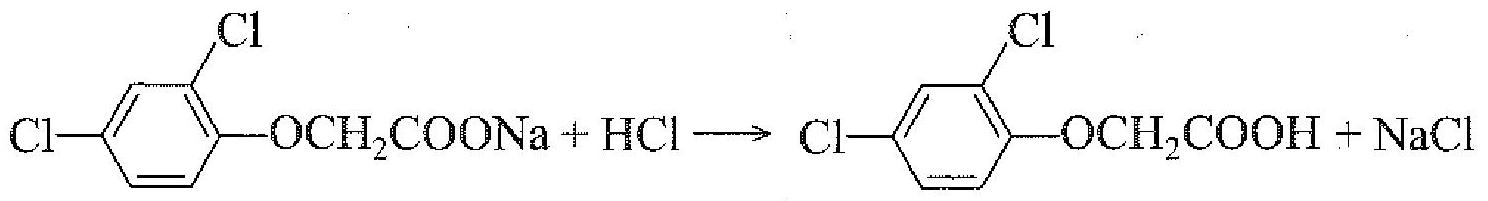
\includegraphics[max width=\textwidth, center]{2025_10_23_052d3249fabea90c1e95g-30(3)}\\
19.19. a)\\
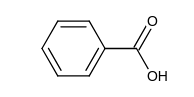
\includegraphics{smile-582d5d3e192bbc73de3bf6a757f7824f5f613dce}\\
b) Do benzoic acid ít tan trong nước nên người ta thường dùng dạng muối sodium. Trong nước, tồn tại cân bằng:\\
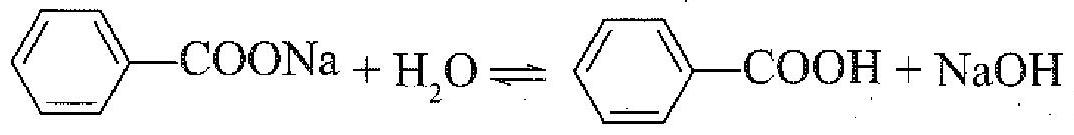
\includegraphics[max width=\textwidth, center]{2025_10_23_052d3249fabea90c1e95g-30(4)}

Benzoic acid sinh ra trong nước với một hàm lượng nhỏ, có tác dụng làm chất bảo quản.\\
c) Tổng hợp benzoic acid từ toluene:

$$
\begin{aligned}
& \mathrm{C}_{6} \mathrm{H}_{5} \mathrm{CH}_{3}+2 \mathrm{KMnO}_{4} \xrightarrow{\mathrm{t}^{\circ}} \mathrm{C}_{6} \mathrm{H}_{5} \mathrm{COOK}+2 \mathrm{MnO}_{2}+\mathrm{KOH}+\mathrm{H}_{2} \mathrm{O} \\
& \mathrm{C}_{6} \mathrm{H}_{5} \mathrm{COOK}+\mathrm{HCl} \xrightarrow{\mathrm{t}^{\circ}} \mathrm{C}_{6} \mathrm{H}_{5} \mathrm{COOH}+\mathrm{KCl}
\end{aligned}
$$

19.20. a) Không chính xác vì trong giấm còn có ethanol hoặc đường còn dư từ theo nguyên liệu để sản xuất.\\
b) Không được, vì nhiệt độ sôi của $\mathrm{CH}_{3} \mathrm{COOH}$ là $118^{\circ} \mathrm{C}$, gần với nhiệt độ sôi của nước.\\
c) Đó là cách thường làm dựa vào phản ứng:

$$
\mathrm{CH}_{3} \mathrm{COOH}+\mathrm{NaOH} \longrightarrow \mathrm{CH}_{3} \mathrm{COONa}+\mathrm{H}_{2} \mathrm{O}
$$

19.21. a) Chỉ có benzoic acid tác dụng được với $\mathrm{NaHCO}_{3}$ do $\mathrm{pK}_{\mathrm{a}}$ (benzoic acid) $<\mathrm{pK}_{\mathrm{a} 2}\left(\mathrm{H}_{2} \mathrm{CO}_{3}\right):$

$$
\mathrm{C}_{6} \mathrm{H}_{5} \mathrm{COOH}+\mathrm{NaHCO}_{3} \rightarrow \mathrm{C}_{6} \mathrm{H}_{5} \mathrm{COONa}+\mathrm{H}_{2} \mathrm{O}+\mathrm{CO}_{2}
$$

b) Trong quy trình đã nêu, phương pháp được sử dụng để tách riêng hai chất benzoic acid và phenol là phương pháp chiết. Chất hữu cơ A thu được từ phần nước là benzoic acid; chất hữu co $\mathbb{B}$ thu được từ phần hữu cơ là phenol.\\
19.22.\\
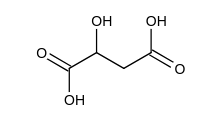
\includegraphics{smile-93d285dd2c97d1c5e4c4b05dbcf44b586dcca220}

malic acid\\
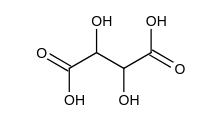
\includegraphics{smile-7bec4bc3248442b90f6ff7e03be18c017abafe98}

tartaric acid\\
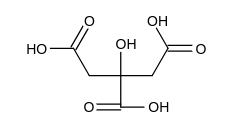
\includegraphics{smile-b5d5d36a8a51bfdedf51c7df504ad53d81b7b0d2}

citric acid\\
19.23*. a) X là\\
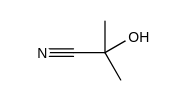
\includegraphics{smile-952464a1491d85cd4b7c5233884a3fdd1e0dd007}\\
b) Y là $\mathrm{NH}_{4} \mathrm{HSO}_{4}$.\\
c) Khối lượng acetone: $10 \cdot 10^{6} \cdot 0,7844=7,844 \cdot 10^{6}(\mathrm{~g})$.

Khối lượng methacrylic acid thu được tính theo lí thuyết:

$$
\frac{7,844 \cdot 10^{6} \cdot 86}{58}=1,163 \cdot 10^{7}(\mathrm{~g})
$$

Vi hiệu suất mỗi giai đoạn là $80 \%$ nên khối lượng methacrylic acid thực thu được:

$$
\frac{1,163 \cdot 10^{7} \cdot 80 \cdot 80 \cdot 80}{100 \cdot 100 \cdot 100}=5,955 \cdot 10^{6}(\mathrm{~g})
$$

Thể tích methacrylic acid thu được là:

$$
\frac{5,955 \cdot 10^{6}}{1,015}=5,867 \cdot 10^{6}(\mathrm{~g})=5,867 \text { tấn. }
$$


\end{document}